\chapter{How to use this book -- some advice for teachers}

If you would like to maximize your students' learning in a field of study that emphasizes critical thinking as much as Instrumentation, I have one simple piece of advice: \textit{engage your students, don't just present information to them}.  Do not make the mistake so many teachers do, of thinking it is their role in the classroom to provide information in pre-digested form to their students, and that it is each student's responsibility to passively absorb this information.

High achievement happens only in an atmosphere of high expectations.  If you design coursework allowing students to expend minimal effort, your students will achieve minimal learning.  Alternatively, if you require students to think deeply about their subject of study, challenge them with interesting and relevant assignments, and hold them accountable to rigorous standards of demonstrated competence, your students can and will move mountains.

In this appendix I present to you some concepts and models for achieving high standards of learning in the field of Instrumentation.  The ideas documented here have all been proven to work in my own instruction, and I continue to use them on a daily basis.  However, this is not a rigid blueprint for success -- I invite and encourage others to experiment with variations on the same themes.  More than anything else, I hope to encourage educators with examples of unconventional thinking and unconventional curricula, to show what may be accomplished if you allow yourself to be creative and results-driven in your instructional design.









\filbreak
\section{Teaching technical theory}

Learning is not merely a process of information transfer.  It is first and foremost a transformation of one's thinking.  When we learn something substantial, it alters the way we perceive and interact with the world around us.  Learning any subject also involves a substantial accumulation of facts in one's memory, but memorization alone is not really learning (at least it isn't learning at the college level).  Transmitting facts into a student's memory is easy, and does not require a live human presenter.  A well-written book or a well-edited video can do a far better and far more consistent job of conveying facts and concepts than any live presentation\footnote{To be sure, there are some gifted lecturers in the world.  However, rather than rely on a human being's live performance, it is better to capture the brilliance of an excellent presentation in static form where it may be peer-reviewed and edited to perfection, then placed into the hands of an unlimited number of students in perpetuity.  In other words, if you think you're great at explaining things, do us all a favor and translate that brilliance into a format capable of reaching more people!}.  A more appropriate role for any human teacher, therefore, is to foster higher-order thinking skills such as problem-solving, logical reasoning, diagnostic techniques, and metacognition (critiquing one's own thinking).

Rather than devote most of your classroom time to lecture-style presentations -- where the flow of information goes primarily from you to your students -- place the responsibility for fact-gathering on your students.  Have them read books such as this\footnote{It would be arrogant of me to suggest my book is the best source of information for your students.  Have them research information on instrumentation from other textbooks, from manufacturers' literature, from whitepapers, from reference manuals, from encyclopedia sets, or whatever source(s) you deem most appropriate.  If you possess knowledge that your students need to know that isn't readily found in any book, \textit{publish it for everyone's benefit!}} and arrive at the classroom \textit{prepared} to discuss what they have already studied.  

When students are with you in the classroom and in the lab, probe their understanding with questions -- lots of questions.  Give them realistic problems to solve.  Challenge them with projects requiring creative thought.  Get your students to reveal how they think, both to you and to their peers.  This will transform your classroom atmosphere from a monologue into a dialogue, where you engage with the minds of your students as partners in the learning process instead of lecturing to them as subordinates.

\vskip 10pt

A format I have used with great success is to assign homework exploring new topics, so students much research those topics in advance of our coverage of it in class.  The pedagogical term for this is an \textit{inverted classroom}, where communication of facts occurs outside of class, and higher-order activities such as problem-solving occur inside the classroom.  This stands in contrast to traditional learning structures, where the instructor spends most of the class time transmitting facts and working example problems, while subsequent homework questions (ostensibly completed on the students' own time) stimulate the development of problem-solving skills.  \index{Inverted classroom}

Homework in my ``inverted'' classroom comes in the form of question sets designed to lead the student on a path to acquiring the necessary facts and exposing them to certain problem-solving techniques.  Some of these questions point students directly to specific texts to read, while others allow students to choose their own research material.  Many of the questions are simply conceptual or quantitative problems to solve, without reference to source materials.  When my students arrive for class, they first take a quiz on the material they should have studied for that day.  After the quiz, students working alone or in small groups solving the assigned problems.  My role as instructor is to assist students in their problem-solving efforts, observing the students' attempts, offering advice, and helping to identify and correct misconceptions.  Students are much more engaged, less distracted, and comfortable raising questions while working together in these groups than they ever are as one large group.

Students are considered finished with the class session (and free to leave) when they are able to successfully demonstrate to me their grasp of the day's material.  This happens in the form of a ``summary quiz'' which may be done one-on-one (my preference) or as a whole class.  If done individually, the summary quizzes must be varied enough so I am adequately challenging each student even though they have overheard classmates answering similar summary quiz questions.

\vskip 10pt

An inverted classroom structure shifts the burden of transmitting facts and concepts from a live teacher to static sources such as textbooks\footnote{And multimedia resources, too!  With all the advances in multimedia presentations, there is no reason why an instructor cannot build a library of videos, computer simulations, and other engaging resources to present facts and concepts to students outside of class time.}.  This shift in responsibility frees valuable class time for more important tasks, namely the refinement of higher-order thinking skills.  It makes no sense to have a subject-matter expert (the instructor) spend most or all of the students' valuable time at school doing what a book or a video could do just as well\footnote{Any instructor who can be replaced with a book or a video \textit{should} be replaced by a book or a video!}.  It is far better to apply that same subject-matter expertise to challenges no book or video can meet: actively identifying student misconceptions, dispensing targeted advice for overcoming difficulties, and stimulating students' minds with follow-up questions designed to illuminate concepts in further detail.

Several important advantages are realized by managing a classroom in this way.  First, the instructor enjoys a privileged view of each students' comprehension, struggles, and misconceptions.  If you are accustomed to teaching in a lecture or other ``stand-up-in-front'' classroom format, you will be utterly amazed to see what your students do and do not comprehend when you watch them dialogue and problem-solve in small groups.  Much of what goes on inside your students' minds is hidden from you when they are seated in neat rows watching you in the front of the classroom.  When students are free to work together in more intimate settings, you get to see how they think, what they understand, and most importantly what they mis-understand.  

Another important advantage of an inverted classroom is how it maximizes your contact with those students who need it most.  Faster students are able to finish their work quickly and leave (or stay in the class to tutor their peers), while the slower students stay to the very end with you until their work is done at their pace.  \textit{When conversing with small groups (3 to 4 students) in the classroom, I spend an average of only 5 to 6 minutes per student to query them on their understanding of the day's material and to challenge them with at least one problem to solve.}  The time saved is incredibly useful, as it allows you to re-structure the topic coverage to include more review, cover additional material, or devote more time to hands-on labwork and projects.

Perhaps the most important benefit of an inverted classroom is that students learn how to independently research, which is no small feat.  In a complex field where technology advances on a daily basis, your students will need to be able to learn new facts on their own (without your assistance!) after they graduate.  Employers have consistently advised me that this is the single most important skill any person can learn in school: how to independently acquire new knowledge and new abilities.  Such a skill not only prepares them for excellence in their chosen career, but it also brings great benefit to every other area of life where the acquisition of new information is essential to decision-making (e.g. participation in the democratic process, legal proceedings, medical decision-making, investing, parenting, etc.).  In this way, the inverted classroom is not just a ``better mousetrap'' but in fact is really catching a ``better mouse.''








\filbreak
\subsection{The problem with lecture}

I speak negatively of lecture as a teaching tool because I have suffered its ineffectiveness from a teacher's perspective for several years.  The problem is not that students cannot learn from an instructor's eloquent presentation; it's that following the lead of an expert's presentation obscures students' perception of their own learning.  Stated in simple terms, \textit{lecture forces every student into the role of spectator when they should be participants.}  Students observing a lecture cannot tell with certainty whether they are actually learning from an expert presentation, or whether they are merely being stimulated.  This is not an obvious concept to grasp, so allow me to elaborate in more detail.

\vskip 10pt

When I began my professional teaching career, I did what every other teacher I knew did: I lectured daily to my students.  My goal was to transfer knowledge into my students' minds, and so I chose the most direct method I knew for that necessary transference of information.  

My first year of teaching, like most teachers' first year, was a trial by fire.  Many days I was lecturing to my students on some subject I had just reviewed (for the first time in a long time) no more than a few days before.  My lesson plans were chaotic to non-existent.  By my second and third years, however, I had developed lesson plans and was thereby able to orchestrate my lectures much more efficiently.  These lesson plans were complete enough to support live demonstrations of concepts during almost every lecture, listing all the materials, components, and equipment I would need to set up in preparation.  If an extensive amount of set-up was required for some demonstration, instructions would be found in lesson plan(s) multiple days in advance in order to give me adequate time.  The result was a very smooth and polished presentation in nearly every one of my lectures.  I was quite proud of the work I had done.

However, I noticed a strange and wholly unintended consequence of all this preparation: with each passing year, my students' long-term recall of concepts presented in lecture seemed to grow worse.  Even my best students, who demonstrated an obvious commitment to their education by their regular study habits, outstanding attendance, and quality work, would shock me by asking me to re-explain basic concepts we had covered in extensive detail months before.  They never complained about the lectures being bad -- quite to the contrary, their assessment of my lectures was always ``excellent'' in my performance surveys.

An increasingly common lament of students as they tried to do the homework was \textit{``I understand things perfectly when you lecture, but for some reason I just can't seem to figure it out on my own.''}  This baffled me, since I had made my presentations as clear as I could, and students seemed engaged and attentive throughout.  It was clear to me as I later worked with these students that often they were missing crucial concepts and/or harbored severe misconceptions, and that there was \textit{no way} things should have made sense to them during lecture given these misconceptions.

Another detail that caught my attention was the fine condition of their textbooks.  In fact, their textbooks were looking better and better with each passing year.  At the conclusion of my first teaching year, my students textbooks looked as though they had been dragged behind a moving vehicle: pages wrinkled, binding worn, and marks scribbled throughout the pages.  As my lectures became more polished, the textbooks appeared less and less used.  My reading assignments were no less thorough than before, so why should the books be used less?

\vskip 10pt

One day I overheard a student's comment that made sense of it all.  I was working in my office, and just outside my door were two students conversing who didn't think I could hear them talking.  One of them said to the other, \textit{``Isn't this class the best?  The lectures are so good, you don't even have to read the book!''}  At the sound of this, my heart sunk.  I began to realize what the problem was, what was needed to fix it, and how I had unwittingly created a poor learning environment despite the best of intentions.

\vskip 10pt

The fundamental problem is this: students observing an expert presentation are fooled into thinking the concepts are easier to grasp and the processes easier to execute than they actually are.  The mastery and polish of the lecturer actually hinders student learning by veiling the difficulty of the tasks.  Matters are no different watching a professional athlete or musician at work: a master makes any task look effortless.  It isn't until you (the spectator) actually try to do the same thing (as a participant) that you realize just how challenging it is, just how much you have to learn, and how much effort you must invest before you achieve a comparable level of proficiency.

When students told me ``for some reason'' they just couldn't seem to solve the same problems I did during lecture ``even though they understood it perfectly'' as I lectured, they were being honest.  This was not some excuse made up to cover a lack of effort.  From their perspective, they truly believed they grasped the concepts while watching me work through them in front of class, and were genuinely mystified why it was so hard for them to perform the same problem-solving tasks on their own.

The simple fact of the matter was that my students did \textit{not} actually grasp the concepts as they watched me lecture.  If they had, the solution of similar problems after lecture should have presented little trouble for them.  Lecture had generated a \textit{false sense of understanding} in their minds.  This made my lectures worse than useless, for not only did they fail to convey the necessary knowledge and skill, but they actually \textit{created an illusion of proficiency} in the minds of my students powerful enough to convince them they did not need to explore the concepts further (by reading their textbooks).  This served to hinder learning rather than foster learning.  

\vskip 10pt

What I needed to do was shatter this illusion if my students were to learn from me more effectively, and especially if they were ever to become independent learners.  Thus began my own personal quest of educational reform.





\filbreak
\subsection{A more accurate model of learning}

A humbling fact every teacher eventually learns is that the depth of a student's learning is primarily a function of the student's effort and not their own.  Even the most dedicated and talented instructor cannot make a student learn if that student does not invest the necessary time and effort.  Conversely, even an unmotivated or incompetent instructor cannot prevent a self-dedicated student from learning on their own.

However, a great many students enter college with the belief that learning is a passive activity: \textit{``It's the instructor's job to give us information -- all we're supposed to do is attend and observe.''}   Unfortunately, this flawed model of learning seems embedded in modern American culture, anchored in students' minds from years of compulsory lecture-based education.  The role of teacher as expert presenter is so relentlessly reinforced that we have difficulty recognizing its flaws, much less conceiving better alternatives.  Teachers choosing to depart from this model invite suspicion and even anger from students accustomed to the status quo of lecture.

One way to help see past one's own biases on a subject is to consider the same (or similar) subject in a different context.  Here, the absurdity of passive learning becomes obvious if we simply switch contexts from academic instruction to athletic instruction.  It would be laughable if a coach or fitness trainer were the one performing all the weight-lifting, sprints, stretching, and practice movements while the student never did anything but observe.  It would be only slightly less humorous if the trainer spent the whole of every session modeling these activities, leaving the student to practice those activities on their own time as ``homework.''  Instead, effective physical training sessions \textit{always} place the student in an active role as soon and as often as possible, so that the instructor's valuable expertise may applied toward identifying errors and recommending corrections.  Instructor-led demonstration is minimized in order to maximize time spent with the student \textit{practicing} their craft.

Academic learning really isn't much different.  If we want students to learn new skills and acquire new mental abilities, students must \textit{practice} those skills and mental processes, and it is during this practice time that an instructor's expertise becomes most valuable.  Accurate self-perception is another reason to immediately engage students in practicing the skills and processes they seek to learn.  When students directly experience just how challenging any concept or task is to master, they immediately recognize how much they have to learn.  This self-awareness is a vital first step to learning, proving the need for committed action on their part.  Only after this recognition is the student psychologically prepared for the hard work of learning.

This is why I favor the ``inverted classroom'' approach.  Students must engage with the new subject(s) \textit{prior} to every classroom session.  From the very moment they arrive, they recognize the challenges of the subject matter, and where they need help understanding it.  With the presentation of facts occurring before class time, the bulk of that time may be spent actually \textit{applying} the concepts instead of \textit{encountering} them.  The relatively mundane task of fact-gathering is relegated to students' time outside of class, while the more challenging and meaningful tasks of problem-solving and analysis happen where the instructor can actually observe and coach.  \index{Inverted classroom}

In order for an inverted classroom structure to work, though, each student must have access to the necessary information in static form (e.g. textbooks, videos, etc.), and be held accountable for doing the necessary preparations.  Access and accountability are absolutely essential to ensuring an inverted classroom will work.  Without the former, students will become frustrated; without the latter, some students won't engage.






\filbreak
\subsection{The ultimate goal of education}

As I have transitioned from a traditional lecturer to a ``reform-minded'' educator, my general philosophy of education has shifted.  My teaching techniques and classroom organization changes preceded this philosophical shift, to be sure, but more and more I am realizing just how important it is to have an educational philosophy, and how such a philosophy helps to guide future reforms.

When I began teaching, my belief was that teaching was a matter of knowledge and skills transference: it was my job as an educator first and foremost to transfer information into my students' minds.  Now, it is my belief that my primary task is to help my students become \textit{autonomous}: able to analyze complex data, turn their thoughts into practical action, and continue learning long after they have left my classroom.  If all I accomplish is helping my students memorize facts, procedures, and formulae about instrumentation, I have utterly failed them.  My real job is to challenge them to become autonomous, critical thinkers and doers, so they will be able to fully take responsibility for their own lives and their own careers.

This shift in philosophy happened as a result of contact with many employers of my students, who told me the most important thing any student could learn in school was \textit{how to learn}.  In life, learning is not an option but a necessity, especially in highly complex fields such as instrumentation and control.  Any instrument technician or engineer who stagnates in their learning is destined for obsolescence.  Conversely, those with the ability and drive to continually learn new things will find opportunities opening for them all throughout their careers.

\vskip 10pt

A former classmate of mine I studied instrumentation with told me of his path to success in this field.  While never the smartest person in class (he struggled mightily with math concepts), he was always very determined and goal-oriented.  His first job placed him in the field of automotive research and development, where he was responsible for ``instrumenting'' heavy trucks with sensors to perform both destructive and non-destructive tests on them.  The instrumentation he used at this job was often quite different from the industrial instruments he learned in school, and so he found himself having to constantly refer to textbooks and equipment manuals to learn how the technology worked.  This was true even when he was ``on the road'' doing field-service work.  He told me of many evenings spent in some tavern or pub, a beer in one hand and an equipment manual in the other, learning how the equipment was supposed to work so he could fix the customer's problem the next day.

This hard work and self-directed learning paid off handsomely for my friend, who went on to set up an entire testing department for a major motorcycle manufacturer, and then started his own vehicle testing company (specializing in power-sport vehicles) after that.  None of this would have been possible for my friend had he relied exclusively on others to teach him what he needed to know, taking the passive approach to learning so many students do.  The lesson is very general and very important: \textit{continual learning is a necessary key to success.}

\vskip 10pt

One of the corollaries to my philosophy of education is that individual learning styles are ultimately not to be accommodated.  This may come as a shock to many educators, who have learned about the various styles of learning (auditory, kinesthetic, visual, etc.) and how the acquisition of new information may be improved by teaching students according to their favored modes.  Please understand that I am not denying the fact different people prefer learning in different ways.  What I am saying is that we fail to educate our students (i.e. empower them with \textit{new} abilities) if all we ever do is teach to their preferences, if we never challenge them to do what is novel or uncomfortable.

The well-educated person can learn by listening, learn by watching others, \textit{and} learn by direct hands-on experimentation.  A truly educated person may still retain a preference for one of these modes over the others, but that preference does not \textit{constrain} that person to learning in only one way.  This is our goal as educators: nothing short of expanding each student's modes of learning.

If a student experiences difficulty learning in a particular way, the instructor needs to engage with that student in whatever mode makes the most sense for them \textit{with the goal of strengthening the areas where that student is weak.}  For example, a student who is weak in reading (visual/verbal) but learns easily in a hands-on (kinesthetic) environment should be shown how to relate what they perceive kinesthetically to the words they read in a book.  Spending time with such students examining an instrument to learn how it functions, then reading the service manual or datasheet for that instrument to look for places where it validates the same principles, is one example of how an instructor might help a student build connections between their strong and weak modes of learning.  Investigating subjects through multiple approaches such as this also shows students the value of each learning mode: a student might find they easily grasp ``how'' an instrument works by directly observing and experimenting with it, but that they more readily grasp ``why'' it was built that way by reading the manufacturer's ``theory of operation'' literature.

\vskip 10pt

Keeping the goal of life-long learning in mind, we must ask ourselves the question of how our students will need to learn new things once they are no longer under our tutelage.  The obvious answer to this question is that they will need to be able to learn in any mode available to them, if they are to flourish.  Life is indifferent to our needs: reality does not adapt itself to favor our strengths or to avoid challenging our weaknesses.  Education must therefore focus on the well-rounded development of learning ability.

By far the greatest amount of resistance I encounter from students in terms of learning styles is learning by reading.  It is rare to find a student who reads well, for example, but struggles at learning in a hands-on environment (kinesthetic) or struggles to understand spoken information (auditory).  The reason for this, I believe, is that reading is a wholly unnatural skill.  Entire cultures exist without a written language, but there is not a culture in the world that lacks a spoken one.  Interpreting the written word, to the level of proficiency required for technical learning, is a skill born of much practice.

Unfortunately, the popular application of learning styles in modern education provides students with a ready-made, officially-sanctioned excuse for not only their inability (``That's just not how my brain works''), but also for continued tolerate of that inability (``I shouldn't have to learn in a way I'm not good at'').  The challenge for the instructor is helping students develop their ability to learn in non-favored modes despite this psychological resistance.

\vskip 10pt

\filbreak

My general advice for educators is to never compromise the ``big picture'' philosophy of empowering your students' thinking.  Some key points I always try to keep in mind are:

\begin{itemize}
\item \textbf{Lead by example:} Regularly showcase for your students your own excitement for the subject and your own continual learning adventures.  Likewise, you need to model the same learning modes you ask them to develop: let them see you learn new things, demonstrating how multiple modes are necessary to be an effective self-educator.
\item \textbf{Teach by asking questions:} Socrates had the right idea -- if you want to make people examine their assumptions and discover misconceptions, ask lots of challenging questions.  This is how I have conditioned myself to respond to student questions: I generally answer with a question of my own seeking the heart of the student's confusion.  Posing ``thought experiments'' for students to conduct is another form of questioning that not only clarifies concepts, but also builds good critical-thinking habits.  Anyone familiar with Socrates' fate knows, however, that people tend to react defensively when their assumptions are challenged by persistent questions.  A helpful hint for avoiding this kind of reaction is to give the student adequate time and personal space to contemplate your questions.  If the student ever feels uncomfortable either with your observation of their efforts or the rapidity of your questioning, they will ``lock up'' and refuse to engage.  Sometimes the best way to manage this behavior is to pose a question to the student, then tell them you will get back to them after a few minutes, rather than to watch them struggle answering your question(s).  \index{Socrates}
\item \textbf{Be willing to provide the help they need:} If students struggle at certain tasks or with thinking in certain ways, devote extra time with them to practice these skills.  Let them know in very practical ways how you are willing to work just as hard as you are asking them to work.  Note that this does not mean giving in to demands for lecture.  That would be giving students what they \textit{want}, rather than what they \textit{need}.  Instead, it means focusing directly on whatever weaknesses are hindering their growth as learners, and aggressively working to strengthen those weaknesses.  If it means reserving time to read with students who say they can't understand the text, then that is your job as their teacher.
\item \textbf{Nothing builds confidence and dissolves apprehension like success:} Remind your students of the challenges they have already overcome, and the progress they have already made.
\item \textbf{Be patient:} That same student who complains now about having to read, to think independently, and tackle challenging problems will come back to thank you years later.  Just as you expected them to think long-term while they were in your class, so you need to think long-term with regard to their appreciation for your standards and efforts.  Transformative education is a marathon, not a sprint!
\end{itemize}







\filbreak
\section{Teaching technical practices (labwork)}

Labwork is an essential part of any science-based curriculum.  Here, much improvement may be made over the ``standard'' educational model to improve student learning.  In my students' Instrumentation courses, I forbid the use of pre-built ``trainer'' systems and lab exercises characterized by step-by-step instructions.  Instead, I have my students construct real working instrumentation systems.  The heart of this approach is a ``multiple-loop'' system spanning as large a geographic area as practically possible, with instruments of all kinds connecting to a centralized control room area.  None of the instruments need perform any practical purpose, since the goal of the multiple-loop system is for students to learn about the instruments themselves.

\label{multiple-loop system}

A model for a multiple-loop system might look something like this:

$$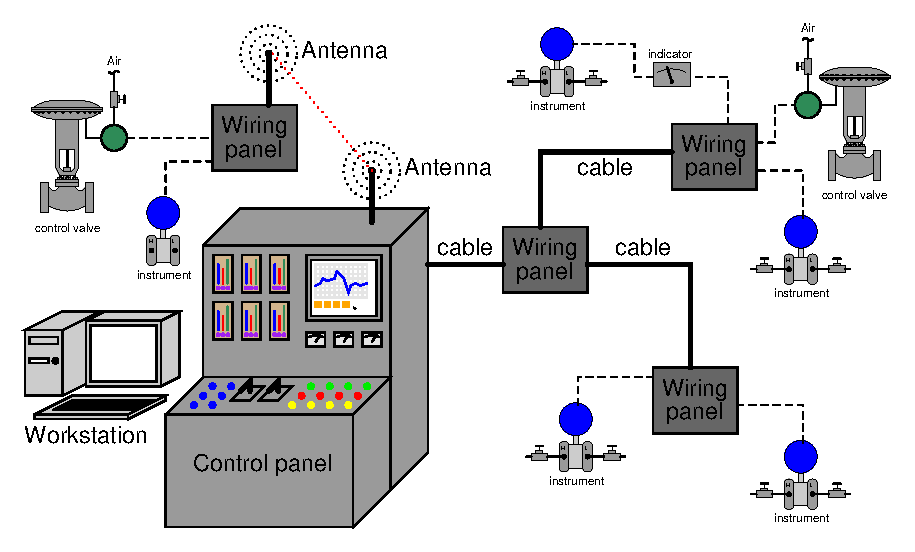
\includegraphics{loop_system.eps}$$

Instruments may or may not be grouped together to form complete control systems, since process control is not necessarily the purpose of this system.  The primary purpose of a multiple-loop instrument system is to provide an infrastructure for students to investigate instrumentation apart from the dynamics of a functioning process.  The separation of controls from process may seem counter-productive at first, but it actually provides a rich and flexible learning experience.  Students are able to measure instrument signals and correlate them with actual physical measurements, take instruments in and out of service, check instrument calibration, see the effects of calibration on measurement accuracy and resolution, practice lock-out and tag-out (LOTO) procedures, diagnose instrument problems introduced by the instructor, practice installing and removing instruments, remove old wire and pull new wire into place, practice sketching and editing loop diagrams, and many other practical tasks without having to balance the needs of a working process.  The system may be altered at any time as needed, since there are no process operating constraints to restrict maintenance operations.  \textit{The fundamental advantage of a process-less instrument system is there are no process limitations restricting educational objectives.  In this sense it is as flexible as a computer simulation, but with the advantage of using real-world components.}  \index{Lock-out, tag-out}  \index{LOTO}

\vskip 10pt

The first academic year I attempted to build such a system with my students was 2002-2003.  Our system cost almost nothing\footnote{Of course, we had to have plenty of instruments to install in this loop system, and industrial instruments are not cheap.  My point is that the \textit{infrastructure} of control panel, trunk cabling, field wiring, terminal blocks, etc. was very low-cost.  If an Instrumentation program already has an array of field instruments for students to work with in a lab setting, it will not cost much at all to integrate these instruments into a realistic multi-loop system as opposed to having students work with individual instruments on the benchtop or installed in dedicated ``trainer'' modules.}, with a control panel fabricated from a discarded fiberglass electrical enclosure and 4-20 mA loop wiring salvaged from discarded spools of category-5 data communications cable (four twisted pairs per cable).  We stapled the cable runs to the lab room wall, and used cheap terminal block assemblies to provide connection points between the cat-5 trunk cables and individual instrument cables.  Our first loops built with this system included the following:

\begin{itemize}
\item Air compressor receiver tank pressure measurement -- \textit{measurement only}
\item Air compressor temperature measurement -- \textit{ measurement only}
\item Regulated (service) air pressure measurement -- \textit{measurement only}
\item Wash basin water level measurement -- \textit{measurement only}
\item Water column level and temperature control -- \textit{measurement and control}
\item Air reservoir pressure control -- \textit{measurement and control}
\end{itemize}

The first four of these instrument loops were ``permanent'' in that they were never disconnected once installed.  The water level and temperature control system was a later addition made toward the end of the academic year.  It began as a pneumatic system, then was upgraded to electronic (single-loop digital controller), then as a PLC-controlled process, then finally as a DCS-controlled process.  The air pressure control system was much the same.  All the time we left the process vessels and field instruments in place, used the same signal tubing and wiring, but merely changed the control instruments at the other end of that tubing and wiring.
 
In addition to these six permanent and semi-permanent loops, students used the system throughout the year to connect individual instruments for loop calibration.  Usually there was no control involved, as they were simply studying individual instruments and were not ready for a complete control system yet.  Every time they had a transducer to calibrate, a control valve to test, or a transmitter to configure, I required them to tie it into the loop system and document the loop using ISA standard loop diagrams.  Then, I would fault their loops (usually electrically by creating opens or shorts in signal wiring, or pneumatically by creating leaks or by plugging tubes with foam earplugs) and have them troubleshoot the loops using real test equipment, documenting their diagnostic steps for grading purposes.  After successful commissioning, calibration, and troubleshooting, students disassembled the loop so the instruments could be used again in a different loop.

Our multiple-loop instrument system -- despite its crude appearance and low cost -- was extremely successful as an educational tool.  My students gained a tremendous amount of practical knowledge and skill in addition to the basic theory.  Abstract principles of measurement and instrument application ``came alive'' for them as they saw the pieces fit together to make a working system.  The intentionally distributed nature of the system -- with the control panel located in one far corner of the room and field instruments scattered around the rest of the room -- forced students to think and work in a manner much more similar to the real work environment.  There were days they were so excited about working on this system that I had to coax them out of class when the school day was over!

\vskip 10pt

In the summer of 2006 I upgraded the loop system to include a 12 foot by 8 foot metal control room panel (donated by a local paper mill), a set of computer workstations for DCS and SCADA system consoles, industry-standard terminal block assemblies located in electrical enclosures, with plenty of electrical conduit runs between different locations in the lab facility to allow pulling of new wires and cables.  Students still must connect each instrument they learn about into the system, configuring either a panel-mounted or computer-based display to register the measured variable in proper units (or to receive a control signal if the instrument in question is a final control element).  Construction of working control systems (transmitter, controller, valve or motor) is quite easy with this infrastructure in place.  The geographically distributed nature of the system lends itself well to realistic troubleshooting, with students working in teams (communicating via hand-held radios) to diagnose problems intentionally placed into the system.

A new feature of the 2006 multi-loop system is that it included digital communication as well as analog (4-20 mA) signaling.  Multiple Ethernet hubs were installed throughout the lab, interconnected to form a single 10 Mbps network linking personal computers with loop controllers and PLCs.  Non-dedicated category 5 cabling was also used for RS-232 and RS-485 communication between serial devices (e.g. data acquisition modules) as needed.  FOUNDATION Fieldbus wiring was also installed (twin-lead shielded cable with 100 $\Omega$ characteristic impedance) allowing the interconnection of fully digital field instruments such as transmitters and digital valve positioners.

\vskip 10pt

The following photographs show the appearance of the new (2006) multiple loop system, beginning with the control panel and computer workstation cluster.  These two elements comprise the ``control room area'' of the lab:

$$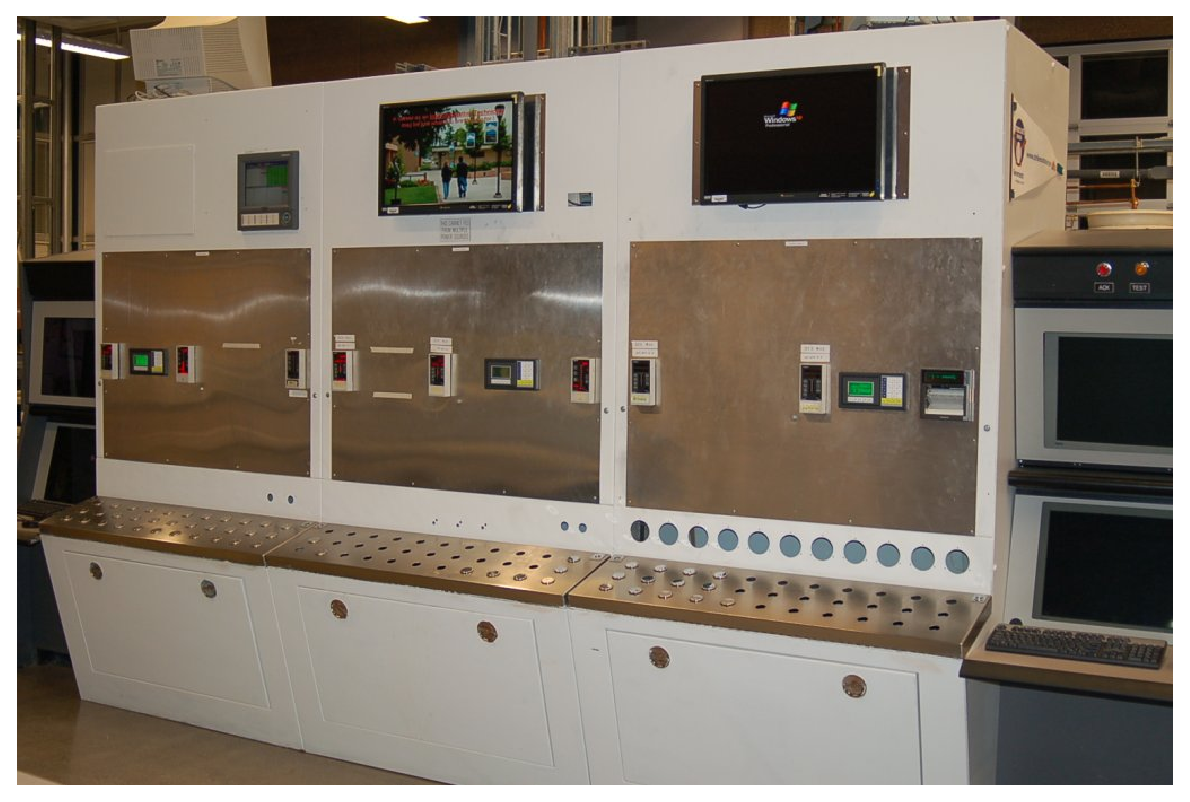
\includegraphics[width=2.5in]{loop_system_3.eps} \hskip 30pt 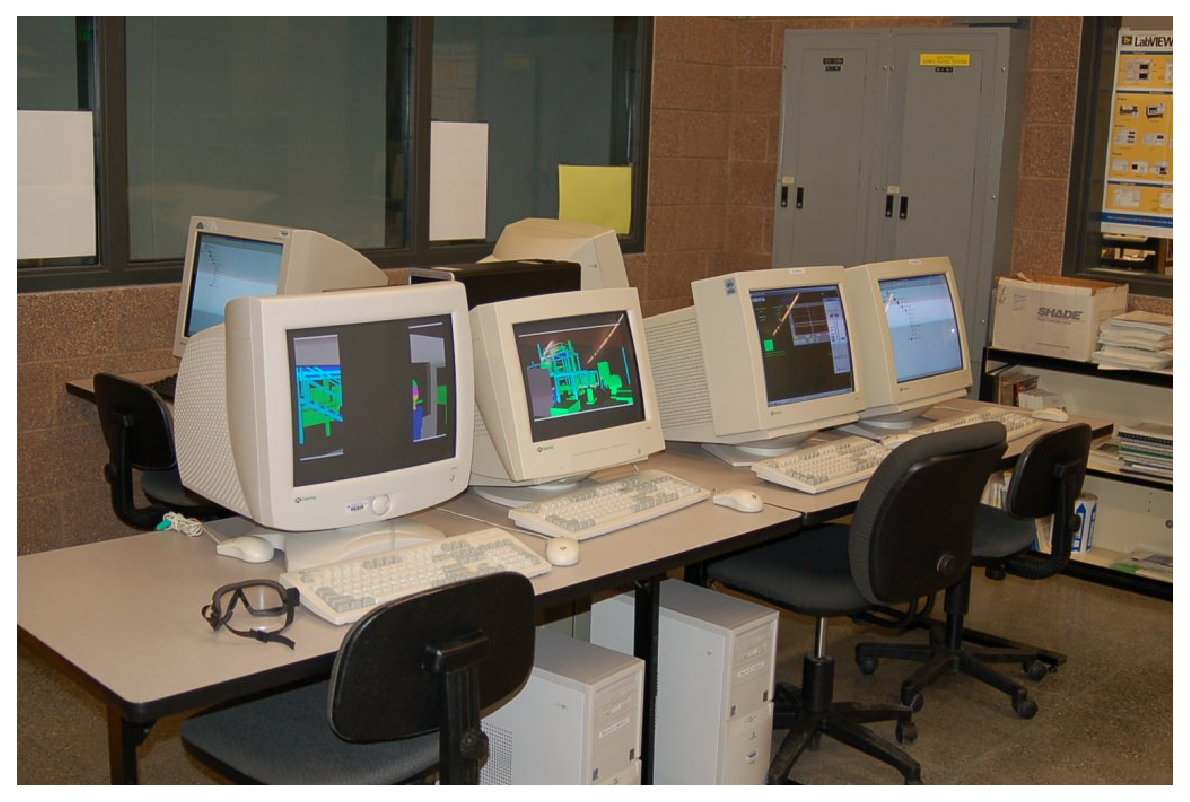
\includegraphics[width=2.5in]{loop_system_5.eps}$$

\filbreak

In another area of the lab room is a pneumatic control panel and a cabinet housing the distributed control system (DCS) I/O rack:

$$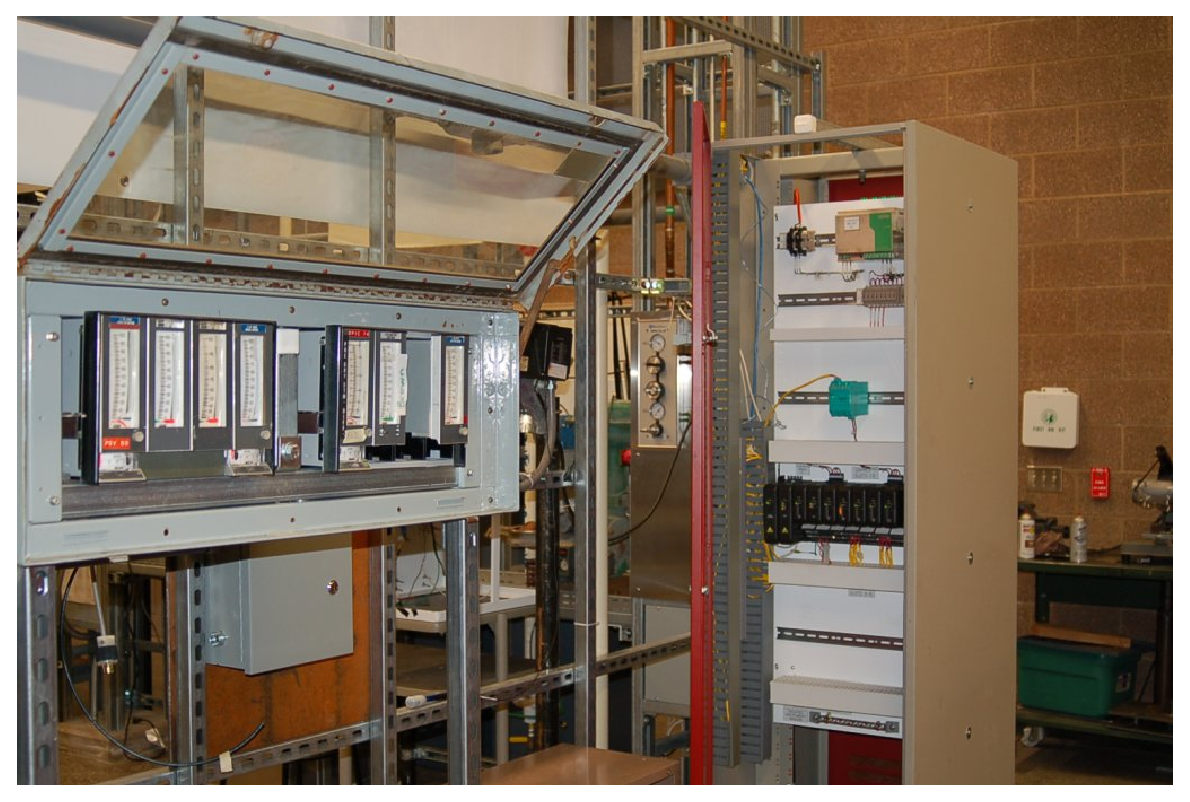
\includegraphics[width=5in]{loop_system_2.eps}$$

\filbreak

The rest of the lab room is dedicated as a ``field area'' where field instruments are mounted and wires (or tubes) run to connect those instruments to remote indication and/or control devices:

$$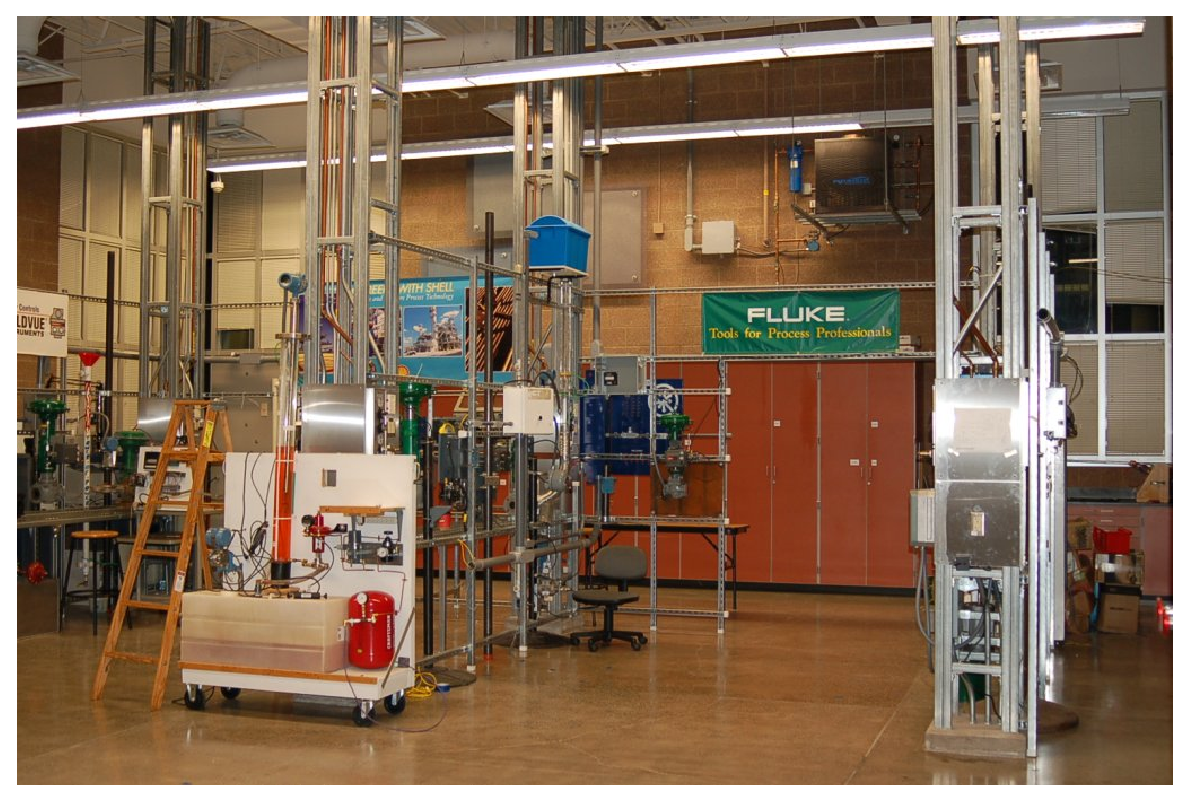
\includegraphics[width=2.5in]{loop_system_1.eps} \hskip 30pt 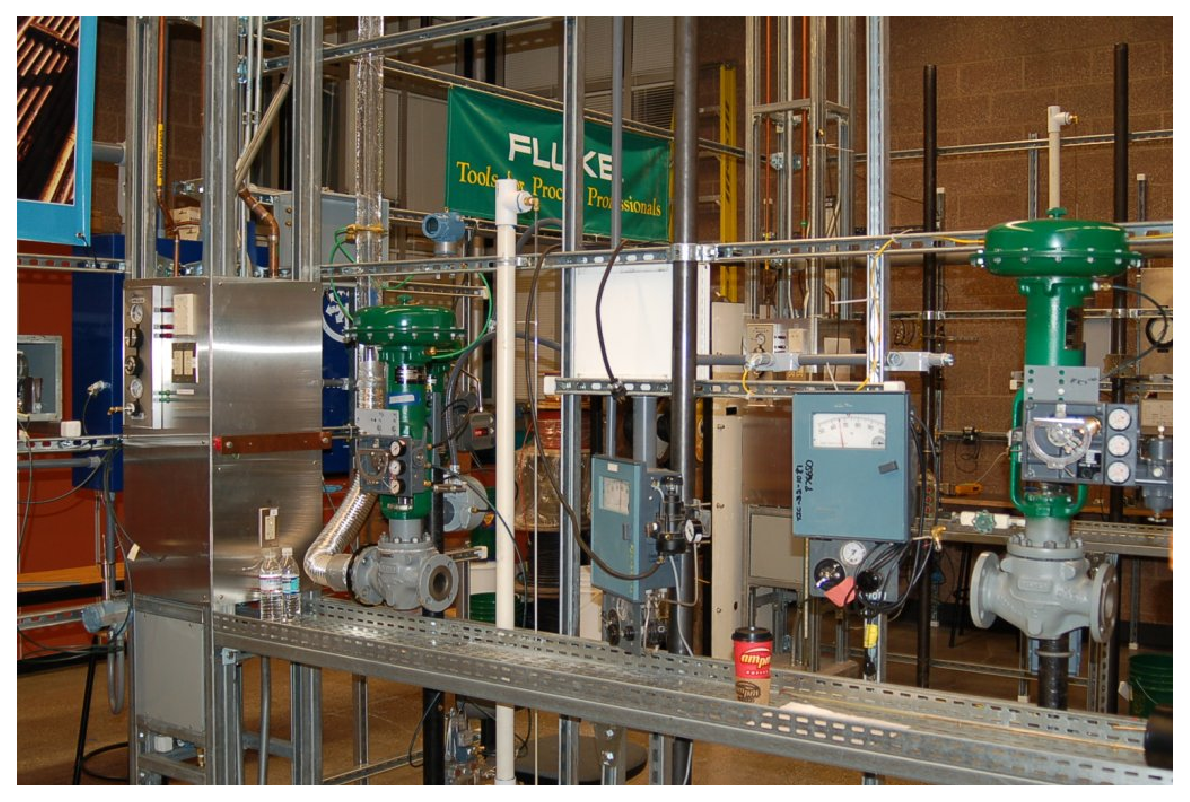
\includegraphics[width=2.5in]{loop_system_4.eps}$$

$$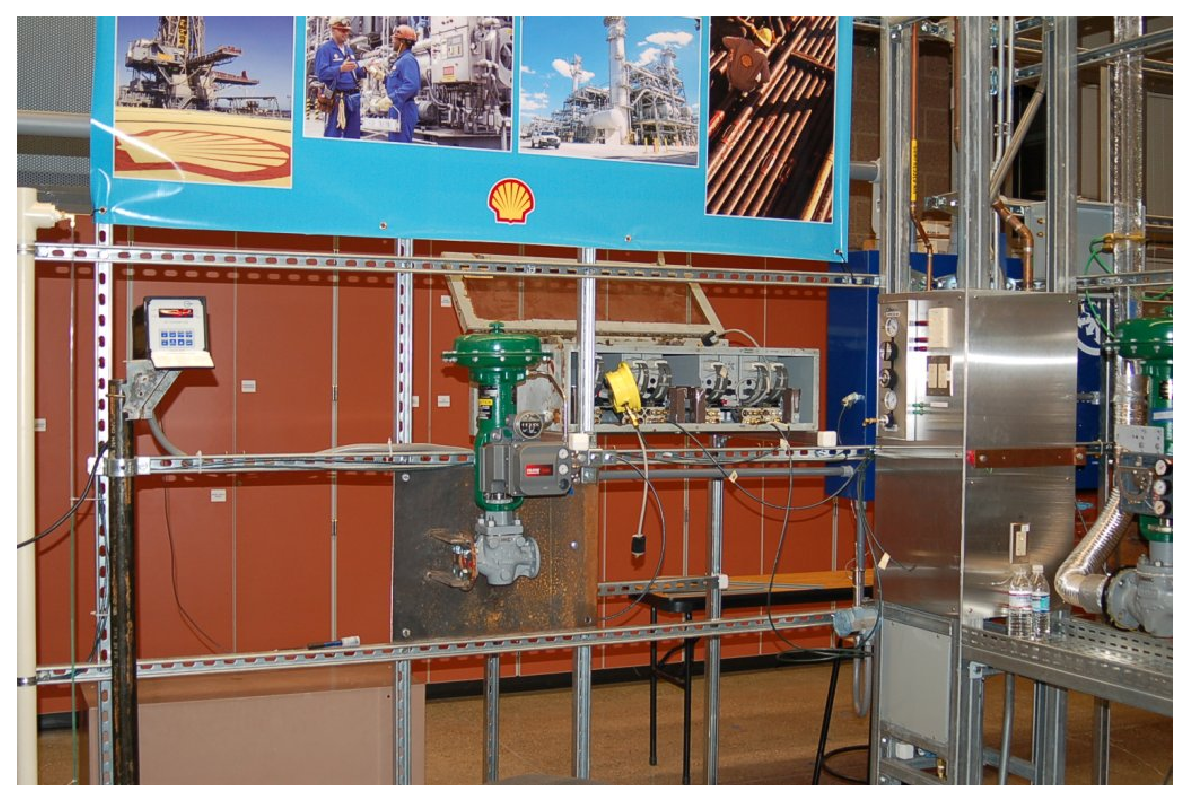
\includegraphics[width=2.5in]{loop_system_6.eps} \hskip 30pt 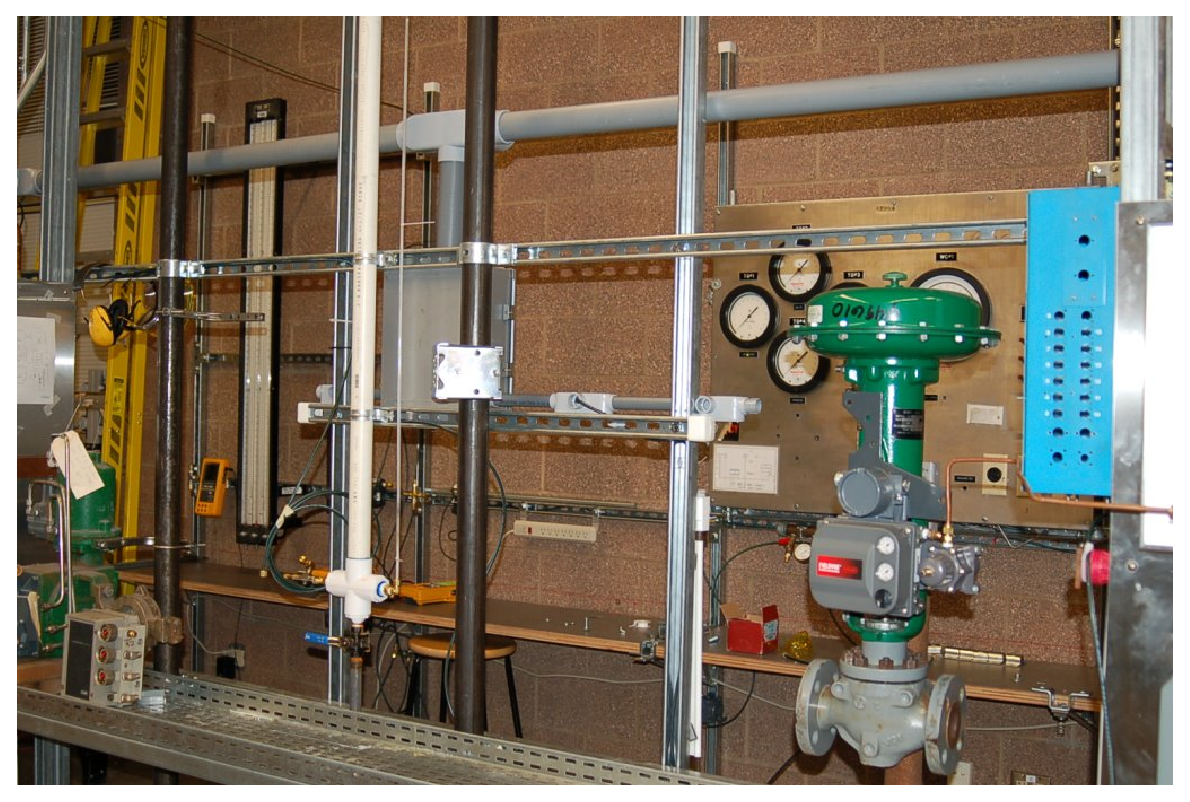
\includegraphics[width=2.5in]{loop_system_7.eps}$$

Note the use of metal strut hardware to form a frame which instruments may be mounted to, and the use of flexible liquid-tight conduit to connect field instruments to rigid conduit pieces so loop wiring is never exposed.  

\filbreak

A less expensive alternative\footnote{When I built my first fully-fledged educational loop system in 2006 at Bellingham Technical College in Washington state (I built a crude prototype in 2003), I opted for Cooper B-Line metal strut because it seemed the natural choice for the application.  It wasn't until 2009 when I needed to expand and upgrade the loop system to accommodate more students that I happened to come up with the idea of using pallet racking as the framework material.  Used pallet racking is plentiful, and very inexpensive compared to building a comparable structure out of metal strut.  As these photographs show, I still used Cooper B-Line strut for some portions, but the bulk of the framework is simply pallet racking adapted for this unconventional application.} to metal strut is standard \textit{industrial pallet racking}, examples shown here with 2 inch pipe attached for instrument mounting, and enclosures attached for instrument cable routing and termination:  \index{Bellingham Technical College}

$$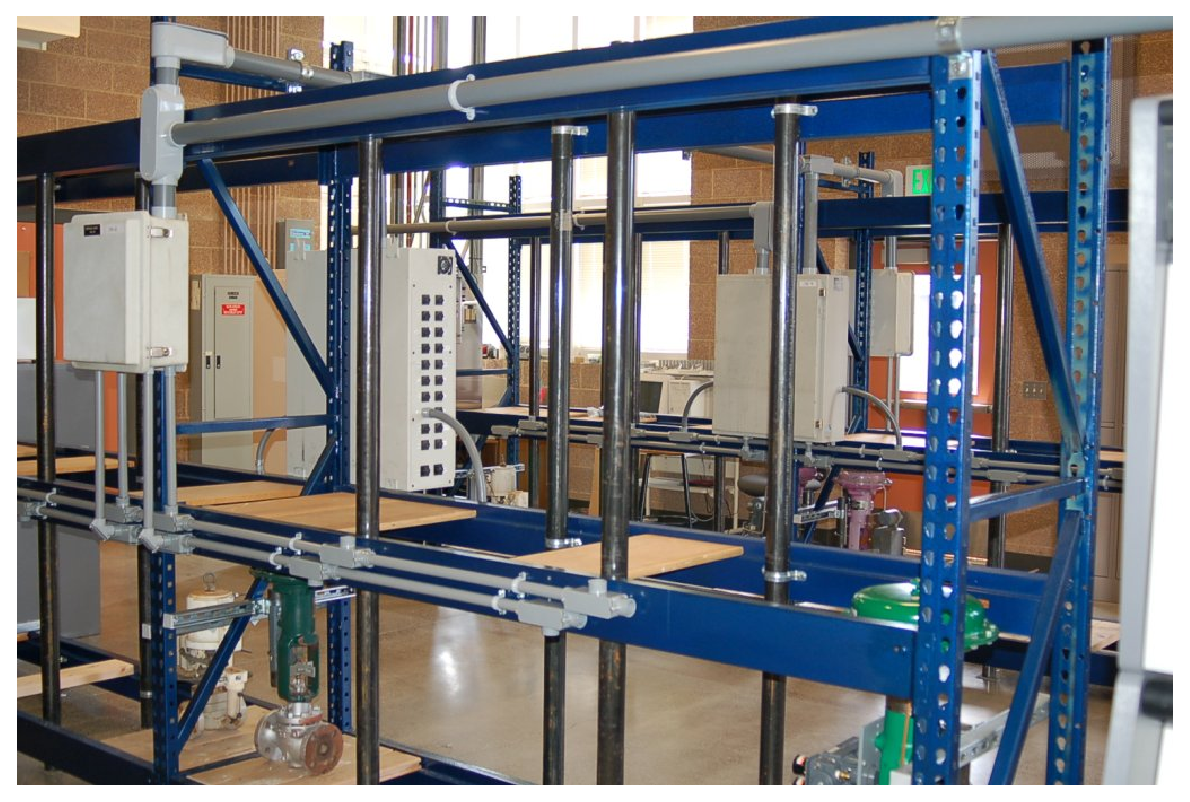
\includegraphics[width=2.5in]{loop_system_8.eps} \hskip 30pt 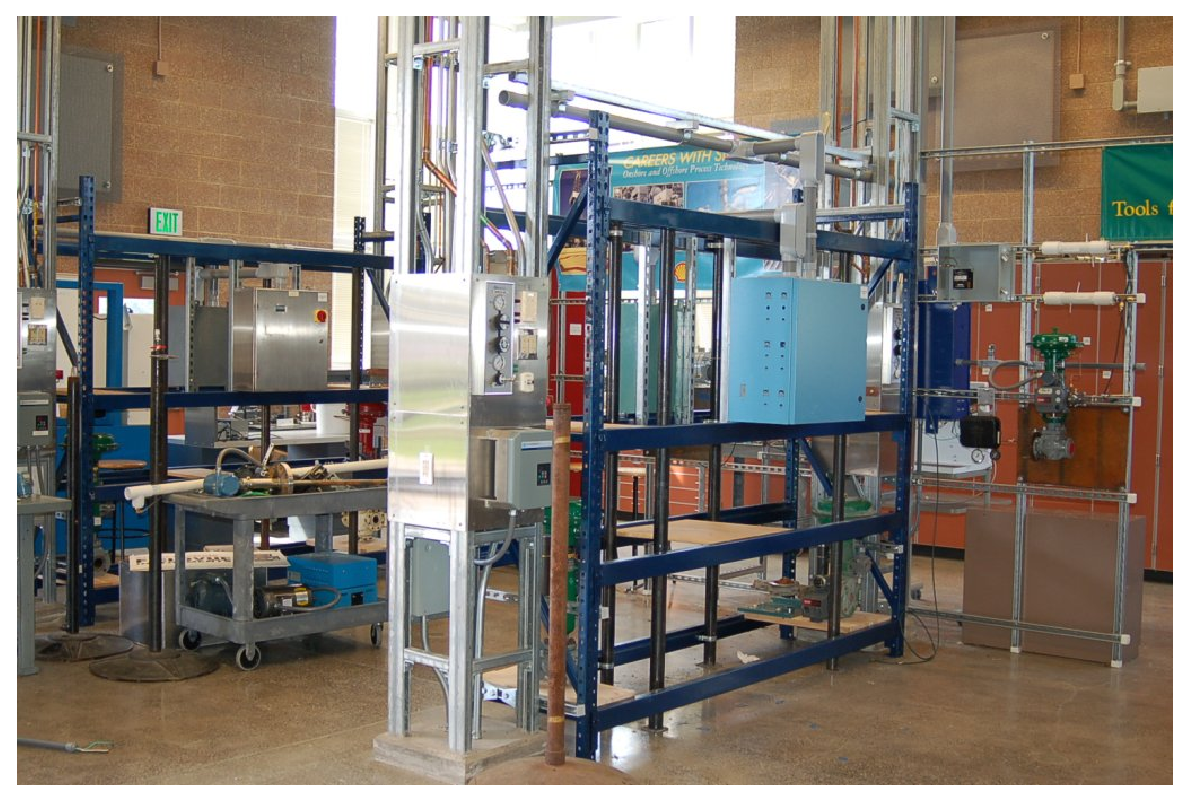
\includegraphics[width=2.5in]{loop_system_9.eps}$$

\vskip 10pt

The multiple-loop system is designed to be assembled, disassembled, and reassembled repeatedly as each student team works on a new instrument.  As such, it is in a constant state of flux.  It is not really a \textit{system} so much as it is an \textit{infrastructure} for students to build working loops and control systems within.

\filbreak

In addition to the multiple-loop system, my students' lab contains working processes (also student-built!) which we improve upon every year.  One such process is a water flow/level/temperature control system, shown here:

$$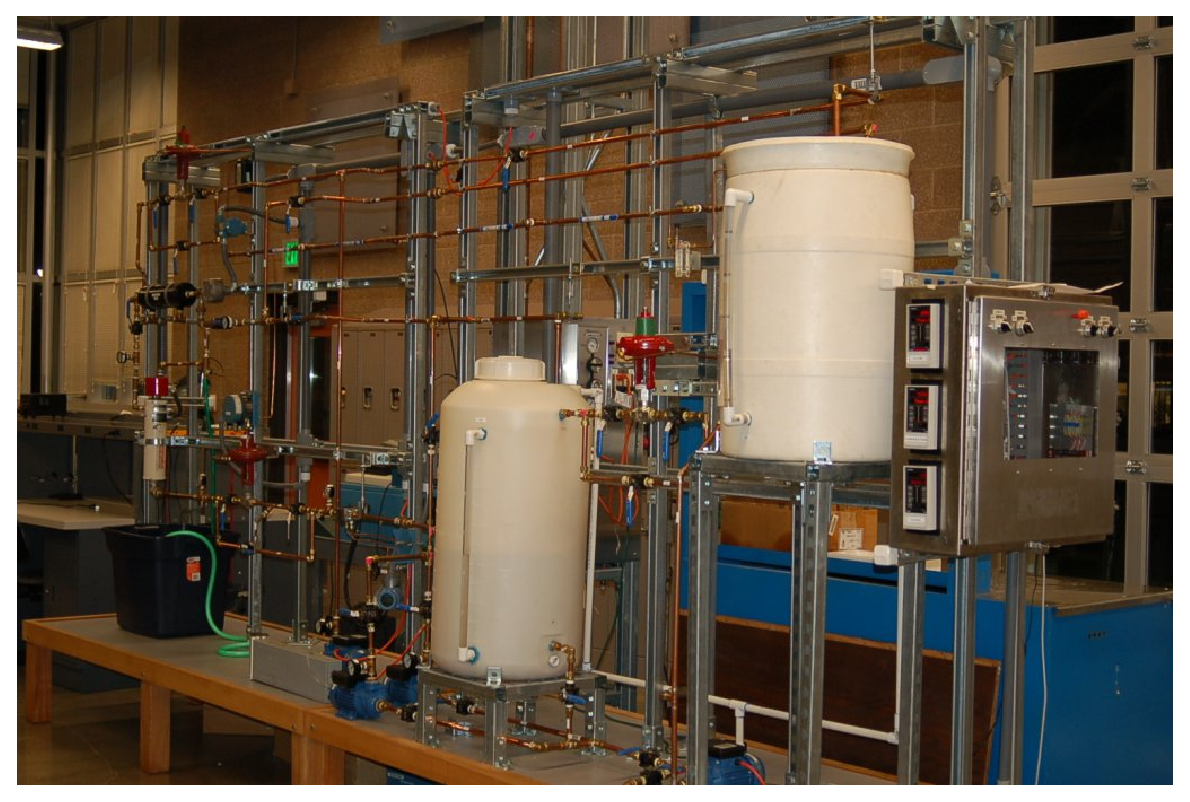
\includegraphics[width=4in]{process_system_1.eps}$$

Another is a turbocompressor system, built around a diesel engine turbocharger (propelled by the discharge of a 2 horsepower air blower) and equipped with a pressurized oil lubrication system and temperature/vibration monitor:

$$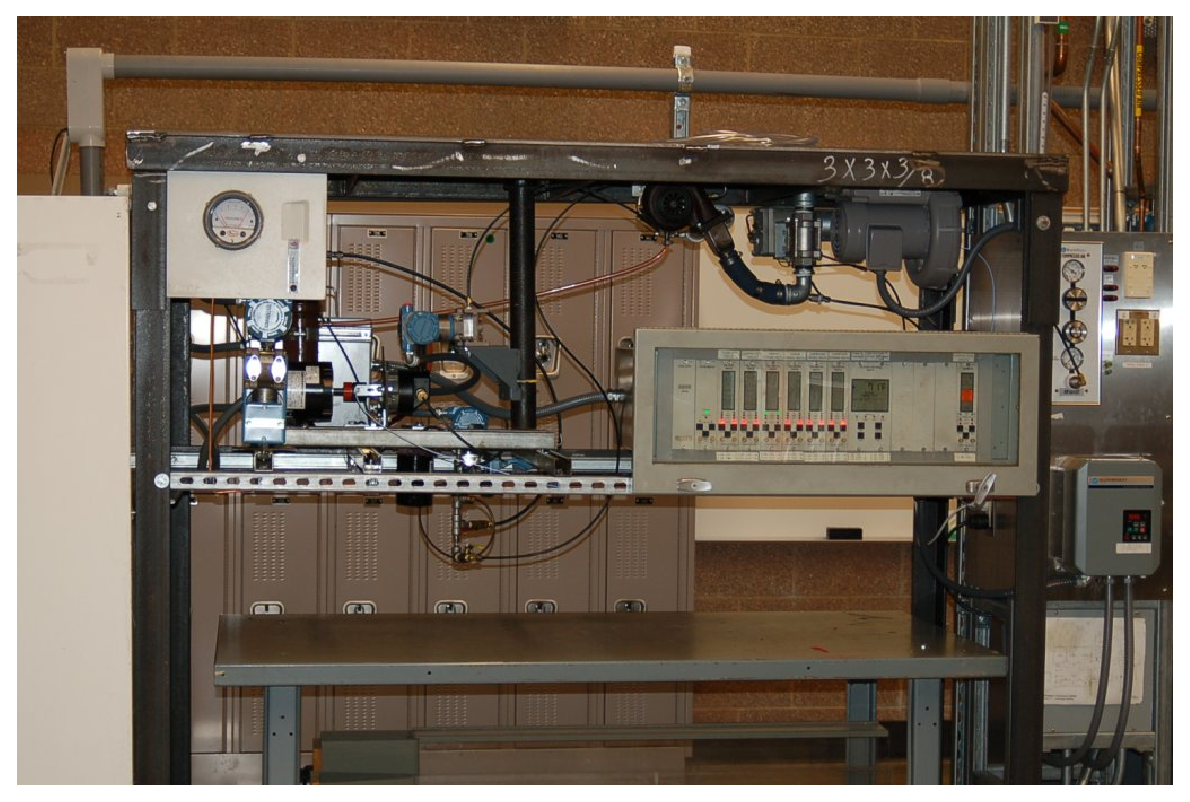
\includegraphics[width=4in]{process_system_2.eps}$$

\filbreak

Yet another permanent process is this electrical power monitoring unit, where protective (overcurrent) relay operation may be demonstrated:

$$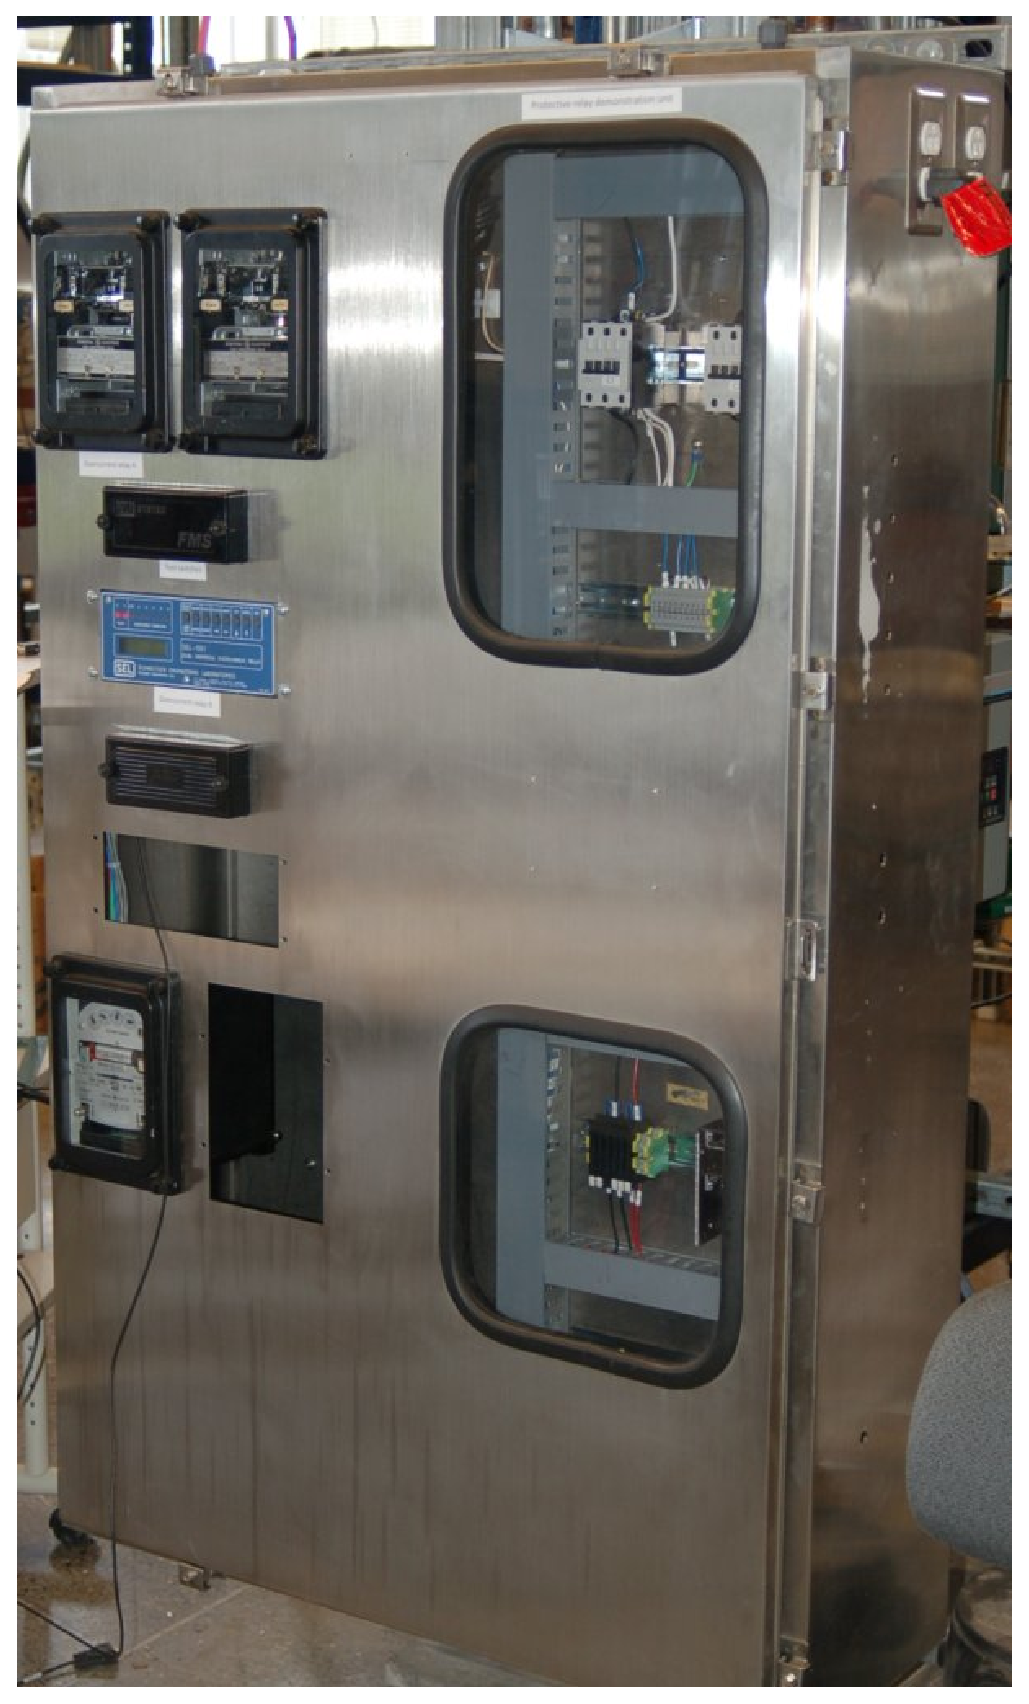
\includegraphics[height=5in]{process_system_3.eps}$$

Measurements of voltage and current in this particular system may be integrated into the rest of the multi-loop system by using voltage and current transducers with 4-20 mA output signals.  Digital protective relays may be connected to the multi-loop system using serial data communication (RS-232, RS-485) signals.

\vskip 10pt

The process piping and equipment on these permanent systems are altered only when necessary, but the control systems on these processes may undergo major revisions each year when a new group of students takes the coursework relevant to those systems.  Having a set of functioning process systems present in the lab at all times also gives students examples of working instrument systems to study as they plan construction of their temporary loops in the multiple-loop system.








\filbreak
\section{Teaching diagnostic principles and practices}

Diagnostic ability is arguably the most difficult skill to develop within a student, and also the most valuable skill a working technician can possess\footnote{One of the reasons diagnostic skill is so highly prized in industry is because so few people are actually good at it.  This is a classic case of supply and demand establishing the value of a commodity.  Demand for technicians who know how to troubleshoot will always be high, because technology will always break.  Supply, however, is short because the skill is difficult to teach.  This combination elevates the value of diagnostic skill to a very high level.}.  In this section I will outline several principles and practices teachers may implement in their curricula to teach the science and art of troubleshooting to their students.

First, we need to define what ``troubleshooting'' is and what it is not.  It is \textit{ not} the ability to follow printed troubleshooting instructions found in equipment user's manuals\footnote{Yes, I have actually heard people make this claim!}.  It is \textit{ not} the ability to follow one rigid sequence of steps ostensibly applicable to any equipment or system problem\footnote{The infamous ``divide and conquer'' strategy of troubleshooting where the technician works to divide the system into halves, isolating which half the problem is in, is but \textit{ one particular procedure: merely one tool in the diagnostician's toolbox}, and does not constitute the whole of diagnostic method.}.  Troubleshooting is first and foremost the practical application of \textit{scientific thinking} to repair of malfunctioning systems.  The principles of hypothesis formation, experimental testing, data collection, and re-formulation of hypotheses is the foundation of any detailed cause-and-effect analysis, whether it be applied by scientists performing primary research, by doctors diagnosing their patients' illnesses, or by technicians isolating problems in complex electro-mechanical-chemical system.  In order for anyone to attain mastery in troubleshooting skill, they need to possess the following traits:

\begin{itemize}
\item  A rock-solid understanding of relevant, fundamental principles (e.g. how electric circuits work, how feedback control loops work)
\item  Close attention to detail
\item  An open mind, willing to pursue actions led by data and not by preconceived notions
\end{itemize}

The first of these points is addressed by any suitably rigorous curriculum.  The other points are habits of thought, best honed by months of practice.  Developing diagnostic skill requires much time and practice, and so the educator must plan for this in curriculum design.  It is not enough to sprinkle a few troubleshooting activities throughout a curriculum, or (worse yet!) to devote an isolated course to the topic.  Troubleshooting should be a topic tested on every exam, present in every lab activity, and (ideally) touched upon in every day of the student's technical education.

Scientific, diagnostic thinking is characterized by a repeating cycle of \textit{inductive} and \textit{deductive} reasoning.  Inductive reasoning is the ability to reach a general conclusion by observing specific details.  Deductive reasoning is the ability to predict details from general principles.  For example, a student engages in deductive reasoning when they conclude an ``open'' fault in a series DC circuit will cause current in that circuit to stop.  That same student would be thinking inductively if they measured zero current in a DC series circuit and thus concluded there was an ``open'' fault somewhere in it.  Of these two cognitive modes, inductive is by far the more difficult because multiple solutions exist for any one set of data.  In our zero-current series circuit example, inductive reasoning might lead the troubleshooter to conclude an open fault existed in the circuit.  However, an unpowered source could also be at fault, or for that matter a malfunctioning ammeter falsely registering zero current when in fact there is current.  Inductive conclusions are \textit{risky} because the leap from specific details to general conclusions always harbor the potential for error.  Deductive conclusions are \textit{safe} because they are as secure as the general principles they are built on (e.g. \textit{if} an ``open'' exists in a series DC circuit, there will be \textit{no} current in the circuit, guaranteed).  This is why inductive conclusions are always validated by further deductive tests, not vice-versa.  For example, if the student induced that an unpowered voltage source might cause the DC series circuit to exhibit zero current, they might elect to test that hypothesis by measuring voltage directly across the power supply terminals.  If voltage is present, then the hypothesis of a dead power source is incorrect.  If no voltage is present, the hypothesis is provisionally true\footnote{Other things could be at fault.  An ``open'' test lead on the multimeter for example could account for both the zero-current measurement and the zero-voltage measurement.  This scientific concept eludes many people: it is far easier to \textit{disprove} an hypothesis than it is to \textit{prove} one.  To quote Albert Einstein, ``No amount of experimentation can ever prove me right; a single experiment can prove me wrong.''}.

Scientific method is a cyclical application of inductive and deductive reasoning.  First, an hypothesis is made from an observation of data (inductive).  Next, this hypothesis is checked for validity -- an experimental test to see whether or not a prediction founded on that hypothesis is correct (deductive).  If the data gathered from the experimental test disproves the hypothesis, the scientist revises the hypothesis to fit the new data (inductive) and the cycle repeats.

Since diagnostic thinking requires both deductive and inductive reasoning, and deductive is the easier of the two modes to engage in, it makes sense for teachers to focus on building deductive skill first.  This is relatively easy to do, simply by adding on to the theory and practical exercises students already engage in during their studies.

\vskip 10pt

Both deductive and inductive diagnostic exercises lend themselves very well to Socratic discussions in the classroom, where the instructor poses questions to the students and the students in turn suggest answers to those questions.  The next two subsections demonstrate specific examples showing how deductive and inductive reasoning may be exercised and assessed, both in a classroom environment and in a laboratory environment. 





\filbreak
\subsection{Deductive diagnostic exercises}

Deductive reasoning is where a person applies general principles to a specific situation, resulting in conclusions that are logically necessary.  In the context of instrumentation and control systems, this means having students predict the consequence(s) of specified faults in systems.  The purpose of building this skill is so that students will be able to quickly and accurately test ``fault hypotheses'' in their minds as they analyze a faulted system.  If they suppose, for example, that a cable has a break in it, they must be able to deduce what effects a broken cable will have on the system in order to formulate a good test for proving or disproving that hypothesis.



\filbreak
\subsubsection{Example: predicting consequence of a single fault}

For example, consider a simple three-resistor series DC circuit, the kind of lab exercise one would naturally expect to see within the first month of education in an Instrumentation program.  A typical lab exercise would call for students to construct a three-resistor series DC circuit on a solderless breadboard, predict voltage and current values in the circuit, and validate those predictions using a multimeter.  A sample exercise is shown here:

$$\includegraphics{trouble01.eps}$$

Note the \textbf{Fault Analysis} section at the end of this page.  Here, after the instructor has verified the correctness of the student's mathematical predictions and multimeter measurements, he or she would then challenge the student to predict the effects of a random component fault (either quantitatively or qualitatively), perhaps one of the resistors failing open or shorted.  The student makes their predictions, then the instructor simulates that fault in the circuit (either by pulling the resistor out of the solderless breadboard to simulate an ``open'' or placing a jumper wire in parallel with the resistor to simulate a ``short'').  The student then uses his or her multimeter to verify the predictions.  If the predicted results do not agree with the real measurements, the instructor works with the student to identify why their prediction(s) were faulty and hopefully correct any misconceptions leading to the incorrect result(s).  Finally, a different component fault is chosen by the instructor, predictions made by the student, and verification made using a multimeter.  The actual amount of time added to the instructor's validation of student lab completion is relatively minor, but the benefits of exercising deductive diagnostic processes are great.  




\filbreak
\subsubsection{Example: predicting consequences of multiple faults}

An example of a more advanced deductive diagnostic exercise appropriate to later phases of a student's Instrumentation education appears here.  A loop diagram shows a pressure recording system for an iso-butane distillation column:

$$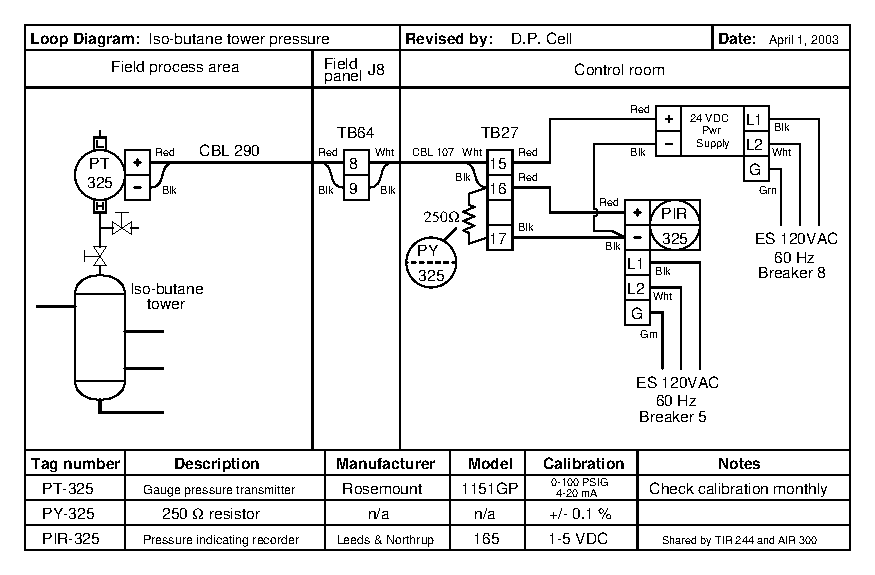
\includegraphics{trouble03.eps}$$

A set of questions accompanying this diagram challenge each student to predict effects in the instrument system resulting from known faults, such as:

\begin{itemize}
\item PT-325 block valve left shut and bleed valve left open (\textit{predict voltage between TB27-16 and TB27-17})
\item Loose wire connection at TB64-9 (\textit{predict pressure indication at PIR-325})
\item Circuit breaker \#5 shut off (\textit{predict loop current at applied pressure of 50 PSI})
\end{itemize}

Given each hypothetical fault, there is only one correct conclusion for any given question.  This makes deductive exercises unambiguous to assess.





\filbreak
\subsubsection{Example: identifying possible faults}

A more challenging type of deductive troubleshooting problem easily given in homework or on exams appears here.  It asks students to examine a list of potential faults, marking each one of them as either ``possible'' or ``impossible'' based on whether or not each fault is independently capable of accounting for all symptoms in the system:

\vskip 20pt

\begin{quotation}

Suppose a voltmeter registers 6 volts between test points \textbf{C} and \textbf{B} in this series-parallel circuit:

\end{quotation}

$$\includegraphics{trouble15.eps}$$

% No blank lines allowed between lines of an \halign structure!
% I use comments (%) instead, so that TeX doesn't choke.

$$\vbox{\offinterlineskip
\halign{\strut
\vrule \quad\hfil # \ \hfil & 
\vrule \quad\hfil # \ \hfil & 
\vrule \quad\hfil # \ \hfil \vrule \cr
\noalign{\hrule}
%
% First row
\textbf{Fault} & \textbf{Possible} & \textbf{Impossible} \cr
%
\noalign{\hrule}
%
% Another row
$R_1$ failed open &  &  \cr
%
\noalign{\hrule}
%
% Another row
$R_2$ failed open &  &  \cr
%
\noalign{\hrule}
%
% Another row
$R_3$ failed open &  &  \cr
%
\noalign{\hrule}
%
% Another row
$R_1$ failed shorted &  &  \cr
%
\noalign{\hrule}
%
% Another row
$R_2$ failed shorted &  &  \cr
%
\noalign{\hrule}
%
% Another row
$R_3$ failed shorted &  &  \cr
%
\noalign{\hrule}
%
% Another row
Voltage source dead &  &  \cr
%
\noalign{\hrule}
} % End of \halign 
}$$ % End of \vbox

\vskip 10pt

This is still a \textit{deductive} thinking exercise because each of the faults is given to the student, and it is a matter of deduction to determine whether or not each one of these proposed faults is capable of accounting for the symptoms.  Students need only apply the general rules of electric circuits to tell whether or not each of these faults would cause the reported circuit behavior.

True to form for any deductive problem, there can only be one correct answer for each proposed fault.  This makes the exercise easy and unambiguous to grade, while honing vitally important diagnostic skills.

\filbreak

One of the benefits of this kind of fault analysis problem is that it requires students to consider \textit{all} consequences of a proposed fault.  In order for one of the faults to be considered ``possible,'' it must account for all symptoms, not just one symptom.  An example of this sort of problem is seen here:

\vskip 20pt

\begin{quotation}

Suppose the voltmeter in this circuit registers a strong \textit{negative} voltage.  A test using a digital multimeter (DMM) shows the voltage between test points \textbf{D} and \textbf{B} to be 6 volts:

\end{quotation}

$$\includegraphics{trouble17.eps}$$

% No blank lines allowed between lines of an \halign structure!
% I use comments (%) instead, so that TeX doesn't choke.

$$\vbox{\offinterlineskip
\halign{\strut
\vrule \quad\hfil # \ \hfil & 
\vrule \quad\hfil # \ \hfil & 
\vrule \quad\hfil # \ \hfil \vrule \cr
\noalign{\hrule}
%
% First row
\textbf{Fault} & \textbf{Possible} & \textbf{Impossible} \cr
%
\noalign{\hrule}
%
% Another row
$R_1$ failed open &  &  \cr
%
\noalign{\hrule}
%
% Another row
$R_2$ failed open &  &  \cr
%
\noalign{\hrule}
%
% Another row
$R_3$ failed open &  &  \cr
%
\noalign{\hrule}
%
% Another row
$R_4$ failed open &  &  \cr
%
\noalign{\hrule}
%
% Another row
$R_1$ failed shorted &  &  \cr
%
\noalign{\hrule}
%
% Another row
$R_2$ failed shorted &  &  \cr
%
\noalign{\hrule}
%
% Another row
$R_3$ failed shorted &  &  \cr
%
\noalign{\hrule}
%
% Another row
$R_4$ failed shorted &  &  \cr
%
\noalign{\hrule}
%
% Another row
Voltage source dead &  &  \cr
%
\noalign{\hrule}
} % End of \halign 
}$$ % End of \vbox

\vskip 10pt

Several different faults are capable of causing the meter to read strongly negative ($R_1$ short, $R_2$ open, $R_3$ open, $R_4$ short), but only two are capable of this while not affecting the normal voltage (6 volts) between test points D and B: $R_3$ open or $R_4$ short.  This simple habit of checking to see that the proposed fault accounts for \textit{all} apparent conditions and not just some of them is essential for effective troubleshooting.

\filbreak

This same question format may be easily applied to most any system, not just electrical circuits.  Consider this example, determining possible versus impossible faults on an exhaust scrubber system:

\vskip 20pt

\begin{quotation}

After years of successful operation, the level control loop in this exhaust scrubbing system begins to exhibit problems.  The liquid level inside the scrubbing tower mysteriously drops far below setpoint, as indicated by the level gauge (LG) on the side of the scrubber.  The operators have tried to rectify this problem by increasing the setpoint adjustment on the level controller (LC), to no avail.  The level transmitter (LT) is calibrated 3 PSI at 0\% (low) level and 15 PSI at 100\% (high) level:

\end{quotation}

$$\includegraphics{trouble16.eps}$$

% No blank lines allowed between lines of an \halign structure!
% I use comments (%) instead, so that TeX doesn't choke.

$$\vbox{\offinterlineskip
\halign{\strut
\vrule \quad\hfil # \ \hfil & 
\vrule \quad\hfil # \ \hfil & 
\vrule \quad\hfil # \ \hfil \vrule \cr
\noalign{\hrule}
%
% First row
\textbf{Fault} & \textbf{Possible} & \textbf{Impossible} \cr
%
\noalign{\hrule}
%
% Another row
Air supply to LT shut off &  &  \cr
%
\noalign{\hrule}
%
% Another row
Air supply to LC shut off &  &  \cr
%
\noalign{\hrule}
%
% Another row
Pump shut off &  &  \cr
%
\noalign{\hrule}
%
% Another row
Broken air line between LT and LC &  &  \cr
%
\noalign{\hrule}
%
% Another row
Broken air line between LC and LV &  &  \cr
%
\noalign{\hrule}
%
% Another row
Plugged nozzle inside LC &  &  \cr
%
\noalign{\hrule}
%
% Another row
Plugged orifice inside LC &  &  \cr
%
\noalign{\hrule}
%
% Another row
Leak in bottom of scrubber &  &  \cr
%
\noalign{\hrule}
} % End of \halign 
}$$ % End of \vbox

\vskip 10pt

This exercise is particularly good because it requires the student to determine the action of the level controller (LC) before some of the proposed faults may be analyzed.  In this case, the level controller must be \textit{direct-acting}, so that an increasing liquid level inside the scrubber will cause an increasing air signal to the air-to-open (ATO) valve. letting more liquid out of the scrubber to stabilize the level.  Without knowing that the level controller is direct-acting, it would be impossible to conclude the effect of a failed air supply to the level transmitter (LT), the first fault proposed in the table.




\filbreak
\subsubsection{Example: assessing value of multiple diagnostic tests}

A variation on this theme of determining the possibility of proposed faults is to assess the usefulness of proposed diagnostic tests.  In other words, the student is presented with a scenario where something is amiss with a system, but instead of selecting a set of proposed faults as being either possible or impossible, the student must determine whether or not a set of proposed \textit{tests} would be diagnostically relevant.  An example of this in a simple series-parallel resistor circuit is shown here:

\vskip 20pt

\begin{quotation}

Suppose a voltmeter registers 0 volts between test points \textbf{E} and \textbf{F} in this circuit.  Determine the diagnostic value of each of the following tests.  Assume only one fault in the system, including any single component or any single wire/cable/tube connecting components together.  If a proposed test could provide new information to help you identify the location and/or nature of the one fault, mark ``yes.''  Otherwise, if a proposed test would not reveal anything relevant to identifying the fault (already discernible from the measurements and symptoms given so far), mark ``no.''

\end{quotation}

$$\includegraphics{trouble18.eps}$$

% No blank lines allowed between lines of an \halign structure!
% I use comments (%) instead, so that TeX doesn't choke.

$$\vbox{\offinterlineskip
\halign{\strut
\vrule \quad\hfil # \ \hfil & 
\vrule \quad\hfil # \ \hfil & 
\vrule \quad\hfil # \ \hfil \vrule \cr
\noalign{\hrule}
%
% First row
\textbf{Diagnostic test} & \textbf{Yes} & \textbf{No} \cr
%
\noalign{\hrule}
%
% Another row
Measure $V_{AC}$ with power applied &  &  \cr
%
\noalign{\hrule}
%
% Another row
Measure $V_{JK}$ with power applied &  &  \cr
%
\noalign{\hrule}
%
% Another row
Measure $V_{CK}$ with power applied &  &  \cr
%
\noalign{\hrule}
%
% Another row
Measure $I_{R1}$ with power applied &  &  \cr
%
\noalign{\hrule}
%
% Another row
Measure $I_{R2}$ with power applied &  &  \cr
%
\noalign{\hrule}
%
% Another row
Measure $I_{R3}$ with power applied &  &  \cr
%
\noalign{\hrule}
%
% Another row
Measure $R_{AC}$ with source disconnected from $R_1$ &  &  \cr
%
\noalign{\hrule}
%
% Another row
Measure $R_{DF}$ with source disconnected from $R_1$ &  &  \cr
%
\noalign{\hrule}
%
% Another row
Measure $R_{EG}$ with source disconnected from $R_1$ &  &  \cr
%
\noalign{\hrule}
%
% Another row
Measure $R_{HK}$ with source disconnected from $R_1$ &  &  \cr
%
\noalign{\hrule}
} % End of \halign 
}$$ % End of \vbox

\vskip 10pt

This form of diagnostic problem tends to be much more difficult to solve than simply determining the possibility of proposed faults.  To solve this form of problem, the student must first determine all possible component faults, and then assess whether or not each proposed test would provide \textit{new information} useful in identifying which of these possible faults is the actual fault.

In this example problem, there are really only a few possible faults: a dead source, an open resistor $R_1$, a shorted resistor $R_2$, a shorted resistor $R_3$, or a broken wire (open connection) somewhere in the loop E-B-A-C-D-F.

The first proposed test -- measuring voltage between points A and B -- would be useful because it would provide different results given a dead source, open $R_1$, shorted $R_2$, or shorted $R_3$ versus an open between A-E or between C-F.  Any of the former faults would result in 0 volts between A and B, while any of the latter faults would result in full source voltage between A and B.

The next proposed test -- measuring voltage between points J and K -- would be useless because we already know what the result will be: 0 volts.  This result of this proposed test will be the same no matter which of the possible faults causing 0 voltage between points E and F exists, which means it will shed no new light on the nature or location of the fault.

\vskip 10pt

Despite being very challenging, this type of deductive diagnostic exercise is nevertheless easy to administer and unambiguous to grade, making it very suitable for written tests.






\filbreak
\subsection{Inductive diagnostic exercises}

Inductive reasoning is where a person derives general principles from a specific situation.  In the context of instrumentation and control systems, this means having students propose faults to account for specific symptoms and data measured in systems.  This is actual troubleshooting, as opposed to deductive diagnosis which is an enabling skill for effective troubleshooting.
 
While real hands-on exercises are best for developing inductive diagnostic skill, much learning and assessment may be performed in written form as well.  





\filbreak
\subsubsection{Example: proposing faults in loop diagram}

This exam question is a sample of an inductive diagnosis exercise presented in written form:

$$\includegraphics{trouble02.eps}$$

\begin{quotation}

This system used to work just fine, but now it has a problem: the controller registers zero flow, and its output signal (to the valve) is saturated at 100\% (wide open) as though it were trying to ``ask'' the valve for more flow.  Your first diagnostic step is to check to see if there actually is gasoline flow through the flowmeter and valve by looking at the rotameter.  The rotameter registers a flow rate in excess of 2 gallons per hour.

Identify possible faults in this system that could account for the controller's condition (no flow registered, saturated 100\% output), depending on what you find when you look at the rotameter:

\vskip 10pt

\begin{itemize}
\item Possible fault:
\item Possible fault:
\end{itemize}

\end{quotation}

Here, the student must identify two probably faults to account for all exhibited symptoms.  More than two different kinds of faults are possible\footnote{Jammed turbine wheel in flowmeter, failed pickup coil in flowmeter, open wire in cable FT-112 or pair 1 of cable 3 (assuming the flow controller's display was not configured to register below 0\% in an open-loop condition), etc.}, but the student need only identify two faults independently capable of causing the controller to register zero flow when it should be registering more than 2 GPH. 





\filbreak
\subsubsection{Example: ``virtual troubleshooting''}

An excellent supplement to any hands-on troubleshooting activities is to have students perform ``virtual troubleshooting'' with you, the instructor.  This type of activity cannot be practiced alone, but requires the participation of someone who knows the answer.  It may be done with individual students or with a group.

\vskip 10pt

A ``virtual troubleshooting'' exercise begins with a schematic diagram of the system such as this, containing clearly labeled test points (and/or terminal blocks) for specifying the locations of diagnostic tests:

$$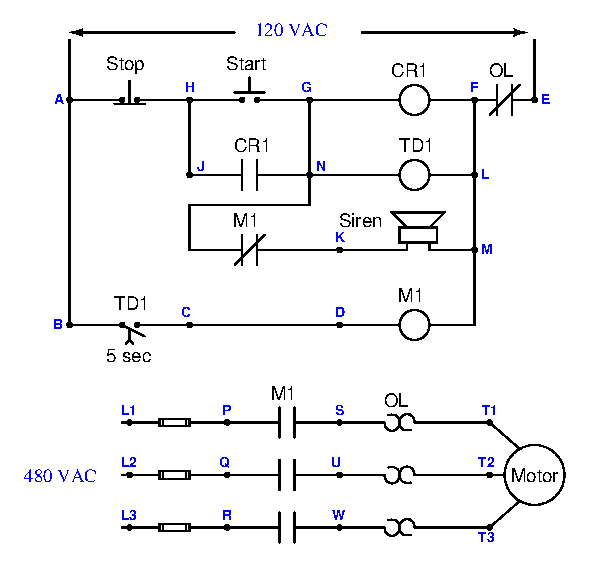
\includegraphics{trouble19.eps}$$

Each student has their own copy of the diagram, as does the instructor.  The instructor has furthermore identified a realistic fault within this system, and has full knowledge of that fault's effects.  In other words, the instructor is able to immediately tell a student how much voltage will be read between any two test points, what the effect of jumpering a pair of test points will be, what will happen when a pushbutton is pressed, etc.

The activity begins with a brief synopsis of the system's malfunction, narrated by the instructor.  Students then propose diagnostic tests to the instructor, with the instructor responding back to each student the results of their tests.  As students gather data on the problem, they should be able to narrow their search to find the fault, choosing appropriate tests to identify the precise nature and location of the fault.  The instructor may then assess each student's diagnostic performance based on the number of tests and their sequence.

When performed in a classroom with a large group of students, this is actually a lot of fun!




\filbreak
\subsubsection{Example: realistic faults in solderless breadboards}

Solderless breadboards are universally used in the teaching of basic electronics, because they allow students to quickly and efficiently build different circuits using replaceable components.  As wonderful as breadboards are for fast construction of electronic circuits, however, it is virtually impossible to create a realistic component fault without the fault being evident to the student simply by visual inspection.  In order for a breadboard to provide a realistic \textit{diagnostic} scenario, you must find a way to hide the circuit while still allowing access to certain test points in the circuit.

A simple way to accomplish this is to build a ``troubleshooting harness'' consisting of a multi-terminal block connected to a multi-conductor cable.  Students are given instructions to connect various wires of this cable to critical points in the circuit, then cover up the breadboard with a five-sided box so that the circuit can no longer be seen.  Test voltages are measured between terminals on the block, not by touching test leads to component leads on the breadboard (since the breadboard is now inaccessible).

\filbreak

The following illustration shows what this looks like when applied to a single-transistor amplifier circuit:

$$\includegraphics{trouble08.eps}$$

If students cannot visually detect a fault, they must rely on voltage measurements taken from terminals on the block.  This is quite challenging, as not even the shapes of the components may be seen with the box in place.  The only guide students have for relating terminal block test points to points in the circuit is the schematic diagram, which is good practice because it forces students to interpret and follow the schematic diagram.







\filbreak
\subsubsection{Example: realistic faults in a multi-loop instrument system}

Whole instrumentation systems may also serve to build and assess individual diagnostic competence.  In my lab courses, students work in teams to build functioning measurement and control loops using the infrastructure of a multiple-loop system (see Appendix section \ref{multiple-loop system} beginning on page \pageref{multiple-loop system} for a detailed description).  Teamwork helps expedite the task of constructing each loop, such that even an inexperienced team is able to assemble a working loop (transmitter connected to an indicator or controller, with wires pulled through conduits and neatly landed on terminal blocks) in just a few hours.

Each student creates their own loop diagram showing all instruments, wires, and connection points, following ISA standards.  These loop diagrams are verified by doing a ``walk-through'' of the loop with all student team members present.  The ``walk-through'' allows the instructor to inspect work quality and ensure any necessary corrections are made to the diagrams.  After each team's loop has been inspected and all student loop diagrams edited, the diagrams are placed in a document folder accessible to all students in the lab area.

Once the loop is wired, calibrated, inspected, and documented, it is ready to be faulted.  When a student is ready to begin their diagnostic exercise, they gather their team members and approach the instructor.  The instructor selects a loop diagram from the document folder \textit{not} drawn by that student, ideally of a loop constructed by another team.  The student and teammates leave the lab room, giving the instructor time to fault the loop.  Possible faults include:

\begin{itemize}
\item Loosen wire connections
\item Short wire connections (loose strands of copper strategically placed to short adjacent terminals together)
\item Cut cables in hard-to-see locations
\item Connect wires to the wrong terminals
\item Connect wire pairs backward
\item Mis-configure instrument calibration ranges
\item Insert square root extraction where it is not appropriate
\item Mis-configure controller action or display
\item Insert unrealistically large damping constants in either the transmitter, indicator, or final element
\item Plug pneumatic signal lines with foam earplugs
\item Turn off hand valves
\item Trip circuit breakers
\end{itemize}

After the fault has been inserted, the instructor calls the student team back into the lab area (ideally using a hand-held radio, simulating the work environment of a large industrial facility where technicians carry two-way radios) to describe the symptoms.  This part of the exercise works best when the instructor acts the part of a bewildered operator, describing what the system is not doing correctly, without giving any practical advice on the location of the problem or how to fix it\footnote{I must confess to having a lot of fun here.  Sometimes I even try to describe the problem incorrectly.  For instance, if the problem is a huge damping constant, I might tell the student that the instrument simply does not respond, because that it what it looks like it you do not take the time to watch it respond \textit{very slowly}.}.  An important detail for the instructor to include is the ``history'' of the fault: is this a new loop which has never worked correctly, or was it a working system that failed?  Faults such as mis-connected wires are realistic of improper installation (new loop), while faults such as loose connections are perfectly appropriate for previously working systems.  Whether the instructor freely offers this ``history'' or waits for the student to ask, it is important to include in the diagnostic scenario because it is an extremely useful piece of information to know while troubleshooting actual systems in industry.  Virtually anything may be wrong (including multiple faults) in a brand-new installation, whereas previously working systems tend to fail in fewer ways.

After this introduction, the one student begins his or her diagnosis, with the other team members acting as scribes to document the student's steps.  The diagnosing student may ask a teammate for manual assistance (e.g. operating a controller while the student observes a control valve's motion), but no one is allowed to help the one student diagnose the problem.  The instructor observes the student's procedure while the student explains the rationale motivating each action, with only a short time given (typically 5 minutes) to determine the general location of the fault causing the problem (e.g. located in the transmitter, control valve, wiring, controller/DCS, tubing, etc.).  If after that time period the student is unable to correctly isolate the general location, the exercise is aborted and the instructor reviews the student's actions (as documented by the teammates) to help the student understand where they went wrong in their diagnosis.  Otherwise, the student is given more time\footnote{The instructor may opt to step away from the group at this time and allow the student to proceed unsupervised for some time before returning to observe.} to pinpoint the nature of the fault.

Depending on the sequencing of your students' coursework, some diagnostic exercises may include components unfamiliar to the student.  For example, a relatively new student familiar only with the overall function of a control loop but intimately familiar with the workings of measurement devices may be asked to troubleshoot a loop where the fault is in the control valve positioner rather than in the transmitter.  I still consider this to be a fair assessment of the student's diagnostic ability, so long as the expectations are commensurate with the student's knowledge.  I would not expect a student to precisely locate the nature of a positioner fault if they had never studied the function or configuration of a valve positioner, but I would expect them to be able to broadly identify the location of the fault (e.g. ``it's somewhere in the valve'') so long as they knew how a control signal is supposed to command a control valve to move.  That student should be able to determine by manually adjusting the controller output and measuring the output signal with the appropriate loop-testing tools that the valve was not responding as it should despite the controller properly performing its function.  The ability to diagnose problems in instrument systems where some components of the system are mysterious ``black boxes'' is a very important skill, because your students \textit{will} have to do exactly that when they step into industry and work with specific pieces of equipment they never had time to learn about in school\footnote{I distinctly remember a time during my first assignment as an industrial instrument technician that I had to troubleshoot a problem in a loop where the transmitter was an oxygen analyzer.  I had no idea how this particular analyzer functioned, but I realized from the loop documentation that it measured oxygen concentration and output a signal corresponding to the percentage concentration (0 to 21 percent) of O$_{2}$.  By subjecting the analyzer to known concentrations of oxygen (ambient air for 21\%, inert gas for 0\%) I was able to determine the analyzer was responding quite well, and that the problem was somewhere else in the system.  If the analyzer had failed my simple calibration test, I would have known there was something wrong with it, which would have led me to either get help from other technicians working at that facility or simply replace the analyzer with a new unit and try to learn about and repair the old unit in the shop.  In other words, my ignorance of the transmitter's specific workings did not prevent me from diagnosing the loop in general.}.

I find it nearly impossible to fairly assign a letter or percentage grade to any particular troubleshooting effort, because no two scenarios are quite the same.  Mastery assessment (either pass or fail, with multiple opportunities to re-try) seems a better fit.  Mastery assessment with no-penalty retries also enjoys the distinct advantage of directing needed attention toward and providing more practice for weaker students: the more a student struggles with troubleshooting, the more they must exercise those skills.  

Successfully passing a troubleshooting exercise requires not only that the fault be correctly identified and located in a timely manner, but that all steps leading to the diagnosis are logically justified.  Random ``trial and error'' tests by the student will result in a failed attempt, even if the student was eventually able to locate the fault.  A diagnosis with no active tests such as multimeter or test gauge measurements, or actions designed to stimulate system components, will also fail to pass.  For example, a student who successfully locates a bad wiring connection by randomly tugging at every wire connection should \textit{not} pass the troubleshooting exercise because such actions do not demonstrate diagnostic thinking\footnote{Anyone can (eventually) find a fault if they check every detail of the system.  Randomly probing wire connections or aimlessly searching through a digital instrument's configuration is not troubleshooting.  I have seen technicians waste incredible amounts of time on the job randomly searching for faults, when they could have proceeded much more efficiently by taking a few multimeter measurements and/or stimulating the system in ways revealing what and where the problem is.  One of your tasks as a technical educator is to discourage this bad habit by refusing to tolerate random behavior during a troubleshooting exercise!}.

\vskip 10pt

To summarize key points of diagnostic exercises using a multiple-loop system:

\begin{itemize}
\item Students work in teams to build each loop
\item Loop inspection and documentation finalized by a ``walk-through'' with the instructor
\item Instructor placement of faults (it is important no student knows what is wrong with the loop!)
\item Each student individually diagnoses a loop, with team members acting merely as scribes
\item Students must use loop diagrams drawn by someone else, ideally diagnosing a loop built by a different team
\item Brief time limit for each student to narrow the scope of the problem to a general location in the system
\item Passing a diagnostic exercise requires:
\subitem $\rightarrow$ Accurate identification of the problem
\subitem $\rightarrow$ Each diagnostic step logically justified by previous results
\subitem $\rightarrow$ Tests (measurements, component response checks) performed before reaching conclusions
\item Mastery (pass/fail) assessment of each attempt, with multiple opportunities for re-tries if necessary
\end{itemize}










\filbreak
\section{Practical topic coverage}

Nearly every technical course teaches and tests students on definitions, basic concepts, and at least some form of quantitative analysis.  If you really intend to prepare your students for the challenges of a career like instrumentation, however, you must cover far more than this.  The following is a list of topics that should be represented in your curriculum every bit as prevalently as definitions, basic concepts, and math:

\begin{itemize}
\item \textit{Qualitative} analysis of instrument systems (e.g. ``Predict how the control system will respond if the flow rate \textit{increases}'')
\item \textit{Qualitative} analysis of processes (e.g. ``Predict what will happen to the pressure in reactor vessel R-5 if valve LV-21 \textit{closes}'')
\item Spatial relations (e.g. mapping wires in a schematic diagram to connection points in a pictorial diagram)
\item Evaluating the validity of someone else's diagnosis of a problem (e.g. ``The last instrument technician to examine this system concluded the problem was a shorted cable.  Based on the data presented here, do you agree or disagree with that conclusion?'')
\item Identification of safety hazards and possible means of mitigation
\item Documentation, both creating it and interpreting it
\item Basic project management principles (e.g. scheduling of time, budgeting material and fiscal resources, limiting project scope, following through on ``loose ends'')
\item Mental math (e.g. approximate calculation without the use of computing equipment)
\item Evaluation of real-life case studies (e.g. students read and answer questions on industry accident reports such as those published by the US Chemical Safety and Hazard Investigation Board)
\end{itemize}

These topics can and should be an explicit -- not implicit -- part of theory and lab (practical) instruction alike.  I do not recommend teaching these topics in separate courses, but rather embedding them within each and every course taught in an Instrumentation program.  By ``explicit'' I mean that these topics should be scheduled for discussion within lesson plans, included within student homework questions, appear as actual questions on exams, and individually demonstrated during labwork.










\filbreak
\section{Principles, not procedures}

One of the marks of a successful problem-solver is a habit of applying general principles to every new problem encountered.  One of the marks of an ineffective problem-solver is a fixation on procedural steps.  Sadly, most of the students I have encountered as a technical college teacher fall into this latter category, as well as a number of working instrument technicians.

Teachers share a large portion of the blame for this sad state of affairs.  In an effort to get our students to a place where they are able to solve problems on their own, there is the temptation to provide them with step-by-step procedures for each type of problem they encounter.  This is a fundamentally flawed approach to teaching, because a set of rigid procedures only works on a very specific set of problems.  To be sure, your students might learn how to solve problems falling within this narrow field by following your algorithmic procedures, but they will be helpless when faced with problems not precisely fitting that same mold.  In other words, they might be able to pass your exams but they will flounder when faced with real-world challenges, and you are utterly wasting their time if you are not preparing them for real-world challenges.

\vskip 10pt

I am as guilty of this as any other teacher.  When I first began teaching (the subject of electronics), I was dismayed at how difficult it was for students to grasp certain fundamental concepts, such as the analysis of series-parallel resistor circuits.  Knowing that I had a very limited amount of time to get my students ready to pass the upcoming exam on series-parallel circuits, I decided to make things simpler for my students by repeatedly demonstrating a set of simple steps by which one could analyze and solve any series-parallel resistor circuit.  Fellow instructors did the same thing, and gladly shared their procedures with me, including tips such as the use of different pen colors (black for drawing wires and components, red for writing current values and directional arrows, and blue for writing voltage values and braces) to help organize all the work.  The procedure could be long-winded depending on how many nested levels of series-parallel resistors were in the circuit, but precisely followed it would never fail to yield the correct answers.  Students greatly appreciated me giving them a set of step-by-step instructions they could follow.

The fallacy of this approach became increasingly evident to me as students would request repeated demonstrations on more and more example problems.  I remember one particular classroom session, after having applied this procedure to at least a half-dozen example problems, that one of the students asked me to do one more example.  \textit{``Are you kidding?''} was the unspoken thought rushing through my mind, \textit{``How many times must you see this demonstrated before you can do it on your own?''}  It suddenly occurred to me that my students were not learning how to solve problems -- instead, they were merely memorizing a sequence of steps including keystrokes on their calculators.  Despite all my effort, the only thing I was preparing them to do successfully was pass the upcoming exam, and that was only because the exam contained exactly the same types of problems I was beating to death on the whiteboard in front of class.

\vskip 10pt

\filbreak

What I should have been doing instead was presenting to my students \textit{only} the general principles of resistor circuits, which may be neatly summarized as such:

\begin{itemize}
\item Ohm's Law ($V = IR$, where $V$, $I$, and $R$ must all refer to the same resistor or same subset of resistors)
\item Resistances in series add to make a larger total resistance ($R_{series} = R_1 + R_2 + \cdots R_n$)
\item Resistances in parallel diminish to make a smaller total resistance ($R_{parallel} = {1 \over {1 \over R_1} + {1 \over R_2} + \cdots {1 \over R_n}}$)
\item Current is the same through all series-connected components
\item Voltage is the same across all parallel-connected components
\end{itemize}

Then, with constant reference to these principles, I should have challenged students to identify where they could be applied to circuits, beginning with the simplest of circuits and progressing to ever-increasing levels of difficulty.

\vskip 10pt

It was not as though I had failed to present these principles often enough, nor that I had failed to demonstrate where these principles applied in the procedure.  My fault was in giving students a comprehensive procedure in the first place, which had the unintended consequence of drawing their attention away from the fundamental principles.  \textit{The simple reason why a step-by-step procedure makes any problem easier to solve is because it eliminates the need for the student to apply general principles to that problem, which is the very thing I my students actually needed to learn.}  To put it bluntly, a comprehensive procedure ``does the thinking'' for the student, because the application of general principles is already pre-determined and encoded into the steps of the procedure itself.  What we get by robotically following the procedure is only an illusion of problem-solving competence.  The real test of whether or not students have mastered the principles (rather than the procedure) is to check their performance on solving similar problems of different form, where the rote procedure is not applicable.

\vskip 10pt

In order to teach students to approach problem-solving from a conceptual rather than procedural perspective, you must insist students show you how they make the links between general principles and the specifics of given problems.  A useful tool for doing this is to have students maintain a notebook identifying and explaining general principles in their own words.  You may choose to allow students the use of their own notepage or notecard on exams, as an incentive to tersely summarize all the major principles they will need to solve problems on exams.  

An inverted classroom structure is well-suited for the encouragement of principle-based problem solving, in that it affords you the opportunity to see how students approach problems and to continually emphasize principles over procedures.









\filbreak
\section{Assessing student learning}

As a general rule, \textit{high achievement only takes place in an atmosphere of high expectations}.  Sometimes these expectations come from within: a self-motivated individual pushes himself or herself to achieve the extraordinary.  Most often, the expectations are externally imposed: someone else demands extraordinary performance.  One of your responsibilities as a teacher is to hold the standard of student performance high (but reasonable!), and this is done through valid, rigorous assessment.

When the time comes to assess your students' learning, prioritize performance assessment over written or verbal response.  In other words, require that your students \textit{demonstrate} their competence rather than merely explain it.  Performance assessment takes more time than written exams, but the results are well worth it.  Not only will you achieve a more valid measurement of your students' learning, but they will experience greater motivation to learn because they know they must put their learning into action.

Make liberal use of \textit{mastery} assessments in essential knowledge and skill domains, where students must repeat a demonstration of competence as many times as necessary to achieve perfect performance.  Not only does this absolutely guarantee students will learn what they should, but the prospect of receiving multiple opportunities to demonstrate knowledge or skill has the beneficial effect of relieving psychological stress for the student.  Mastery assessment lends itself very well to the measurement of diagnostic ability.

An idea I picked up through a discussion on an online forum with someone from England regarding engineering education is the idea of breaking written exams into two parts: a \textit{mastery} exam and a \textit{proportional} exam.  Students must pass the mastery exam(s) with 100\% accuracy in order to receive a passing grade for each course, while the proportional exam is graded like any regular exam (with a score between 0\% and 100\%) and contributes to their letter grade\footnote{It should be noted that some incentive ought to be built in to the mastery exams, or else students will tend to not study for them (knowing they can always retest with no penalty).  This incentive may take the form of time (e.g. mastery re-takes compete for time needed to complete other coursework) and/or take the form of a percentage score awarded on each student's \textit{first attempt} on that exam.}.  Students are given multiple opportunities to pass each mastery exam, with different versions of the mastery exam given at each re-take.  Mastery exams cover all the basic concepts, with very straight-forward questions (no tricks or ambiguous wording).  The proportional exam, by contrast, is a single-effort test filled with challenging problems requiring high-level thinking.  By dividing exams into two parts, it is possible to guarantee the entire class has mastered basic concepts while challenging even the most capable students.

Another unconventional assessment strategy is to create multi-stage exams, where the grade or score received for the exam depends on the highest level passed.  I have applied this to the subject of PLC programming: a large number of programming projects are provided as examples, each one fitting into one of four categories of increasing difficulty.  The first level is the minimum required to pass the course, while the fourth level is so challenging that only a few students will be able to pass it in the time given.  For each of these levels, the student is given the design parameters (e.g. ``program a motor start-stop system with a timed lockout preventing a re-start until at least 15 seconds has elapsed''); a micro-PLC; a laptop computer with the PLC programming software; the necessary switches, relays, motors, and other necessary hardware; and 1 hour of time to build and program a working system.  There are too many example projects provided for any student to memorize solutions to them all, especially when no notes are allowed during the assessment (only manufacturer's documentation for the PLC and other hardware).  This means the student must demonstrate both mastery of the basic PLC programming and wiring elements, as well as creative design skills to arrive at their own solution to the programming problem.  There is no limit to the number of attempts a student may take to pass a given level, and no penalty for failed efforts.  Best of all, this assessment method demands little of the instructor, as the working project ``grades'' itself.

\vskip 10pt

My philosophy on assessment is that good assessment is actually more important than good instruction.  If the assessments are valid and rigorous, student learning (and instructor teaching!) will rise to meet the challenge.  However, even the best instruction will fail to produce consistently high levels of student achievement if students know their learning will never be rigorously assessed.  In a phrase, \textit{assessment drives learning}.

For those who might worry about an emphasis on assessment encouraging teachers to ``teach to the test,'' I offer this advice: there is nothing wrong with teaching to the test so long as the test is valid!  Educators usually avoid teaching to the test out of a fear students might pass the test(s) without actually learning what they are supposed to gain from taking the course.  If this is even possible, it reveals a fundamental problem with the test: it does not actually measure what you want students to know.  A valid test is one that cannot be ``foiled'' by teaching in any particular way.  Valid tests challenge students to think, and cannot be passed through memorization.  Valid tests avoid asking for simple responses, demanding students articulate reasoning in their answers.  \textit{Valid tests are passable only by competence.}

\vskip 10pt

Another important element of assessment is long-term review.  You should design the courses in such a way that important knowledge and skill areas are assessed on an ongoing basis up through graduation.  Frequent review of foundational concepts is a best practice for attaining mastery in any domain.











\filbreak
\section{Common educational fallacies}

When I began teaching full-time in 1998, most of what I thought I understood about good teaching was actually wrong.  Some of this was due to ignorance and inexperience on my part, but a lot of what I thought was good teaching was nothing more than convention.  I reflected on my experiences as a student and believed that was a sufficient model to follow as a teacher.

\vskip 10pt

The following subsections are all titled with fallacies I have held and/or witnessed in others.  Within each subsection I describe the fallacy and then explain why it is fallacious.



\subsection{Fallacy: the sufficiency of presentation}

A common fallacy in education is that clear presentation is sufficient for learning.  While it is important to present information very clearly and accessibly, this surprisingly is not as important as one might think.  It becomes even less important as the student grows in their ability to seek and absorb information on their own.

In fact, it is actually possible for presentations to be \textit{too clear} for their own good.  A presentation of information that makes complete and perfect sense at the first encounter may lull the receiver into believing the topic is simpler than it is.  A presentation that does not inspire follow-up questions has failed to achieve its ultimate goal, which is to foster the critical thinking necessary to become an autonomous learner.





\subsection{Fallacy: you need a well-equipped lab}

Whenever an educational institution offers tours of a new program, the first stop on the tour is always the laboratory where students apply their learning.  This is especially true for technical programs such as Instrumentation.  A school will brag about how much money they spent to equip the facility, how modern the components and tools are, and how similar the lab environment is to the intended work environment.  Surprisingly, almost none of these things matter.

I learned this important lesson by teaching at a college starved of resources.  I simply could not afford to purchase modern lab equipment, and so I was forced to make do with equipment we built ourselves.  What I discovered in this process is that a site-built system offers more learning than one that is pre-packaged and typically costs an order of magnitude more.  This is especially true if students get involved in the design and construction of the lab system(s), because they see the entire development process rather than just the finished product.

This is not to say that all lab facilities may be built on a shoestring budget.  For some topics of study there simply is no choice but to invest in the right (expensive) equipment.  However, what matters most is how you \textit{use} that equipment.  The best-equipped lab is nearly useless without the right assignments and exercises to challenge students on its use; with the right curriculum in place, however, even a meager lab will yield phenomenal learning.

\vskip 10pt

I especially urge caution to technical educators considering the purchase of pre-built ``trainer'' units, which are offered by a number of manufacturers (e.g. Festo, Lab-Volt, Hampden Engineering, etc.) at exorbitant prices.  In almost every case it is possible to build your own equivalents to these trainer units at a mere fraction of the cost, and with greater gains in learning.







\subsection{Fallacy: teach what they'll most often do}

This fallacy is frequently seen in \textit{skill standards} generated by industry and educational organizations: job tasked are ranked by frequency (i.e. how often an employee will have to perform that task) with the implication that the curriculum should mirror that frequency.  This is just nonsense, and for the simplest of reasons: if a task is frequently performed on the job, then the new employee will readily learn that task by working that job.  In other words, the repetitive nature of the task naturally translates into on-the-job training (OJT) and renders any time spent on those tasks in formal education rather questionable.  \index{OJT}  \index{On-the-job training}

It should be rather obvious that the purpose of formal education for the workplace is to teach students how to do things that are \textit{not} easily learned on the job.  Otherwise, why not just hire in as an apprentice and learn your trade entirely by working it?

\vskip 10pt

What skill standard surveys and other rankings of job tasks ought to do is sort these job functions both by importance and by how difficult they are to learn.  When building a formal curriculum, you should first identify which of the tasks rank high in important, then skip (or only touch on) the easy stuff and focus aggressively on those important tasks that are difficult to master.







\subsection{Fallacy: successful completion equals learning}

Students are masters at figuring out how to maximize the grade-to-effort ratio.  This is one problem they know full well how to solve.  In recognizing this fact, we as educators must ensure the tasks we give them to complete cannot be completed unless and until the desired learning occurs.

A good example of this is any mathematical problem given to students to solve.  Suppose the correct answer consists of a number or a formula.  If a student completes the activity by presenting the correct formula, does it mean they actually understand the intended principles of this problem?  It is surprisingly difficult to design valid learning activities and assessments due to the difficulty of discerning another person's understanding.  Perhaps the student is able to arrive at the same correct answer through incorrect reasoning.  Perhaps they copied the result from a classmate.  Perhaps they just made a \textit{guess}, which is likely when the answer consists of selecting between a few choices.






\subsection{Fallacy: teamwork}

The ability to function well on a work team is obviously important, and should be nurtured along with other interpersonal skills and habits in any educational program aiming to place graduates into the workforce.  However, teamwork is far from ideal as a \textit{method of instruction}.  The reason for this is quite simple: students tend to help one another in ways that do not lead to genuine learning, even when their intent is pure.  What you will almost always find in team environments is that the goal of the team is to \textit{complete the task}, not to \textit{ensure education of its members}.  This is really the ``Successful completion equals learning'' fallacy in a different form.  For those of you who have taught before with students working in teams, how often do you see a team collectively decide to sacrifice their group progress for the sake of ensuring a weaker teammate learns an important concept?  I'll wager this is a rare event in any teacher's experience.

Moreover, teamwork masks individual student weaknesses from the instructor's sight.  If a student is weak in one or more areas of their understanding, this deficit stands in hard relief when the student must individually demonstrate their understanding, but is all but hidden when all you see is the product of the group.  

From my own practice as an instructor, I have found that when students are forced by circumstance to complete a task normally reserved for a team, the learning is vastly greater.  No longer can a student rely on the strengths of their peers, and because of this the student must address their own weaknesses directly.





\subsection{Fallacy: tutoring as a panacea}

When a student's grades fall below normal, a common instinct among educators is to provide some form of tutoring to that student.  Tutoring sessions often consist of one-on-one meetings with a qualified person to review whatever subject(s) are posing the problem.  The problem with this seemingly rational response is that tutoring usually resembles the worst form of instruction: enhancing the presentation of information without enhancing the degree or type(s) of challenge.

Tutoring can be useful, but only when properly executed and assigned to the correct students.  There are many ways in which students may be ill-suited to benefit from tutoring.  One example I have witnessed too many times is when a student struggles with coursework for non-cognitive reasons such as outside stress, lack of motivation, or poor judgment and/or personal habits.  The key to successful tutoring is to first diagnose the true nature of the impediment hampering a student's progress, and then connecting the student to the right tutor only if that is what will actually help them.






\subsection{Fallacy: learning styles}

Much could be said on this currently popular topic.  It seems one cannot read any modern literature on student learning without encountering something about learning styles: the notion that each person absorbs information best in unique ways, and therefore optimum instruction tailors its presentation on a style-by-style basis\footnote{This latter concept is called the \textit{mesh hypothesis}: that learning is enhanced when one's learning style meshes well with instruction given in that style}.  I will not attempt to deconstruct the various theories of learning styles, for I am not qualified to do so.  What I \textit{will} do, though, is highlight the fallacy of learning styles as they are commonly practiced.

When a student explains to me as their instructor that they have a specific learning style, it is always in the context of a larger discussion about why they are struggling to learn something.  In other words, their learning style is not being accommodated, and that's why they are experiencing trouble in school.  A few errors usually surface at this point:

\begin{enumerate}
\item The first error is confusion of what learning styles are even supposed to be.  The most common scenario I encounter as an instructor is that the student claims it's difficult for them to learn new information by reading,\textit{because they are a ``visual'' learner and must see a concept being demonstrated in order to grasp it}.  This has always struck me as odd, since reading is an intrinsically visual activity (unless one reads in Braille).  The real problem is that the student is not adept at extracting ideas from text, and this is a \textit{reading deficit}.  What they are essentially claiming is that they cannot learn anything new without some other person showing it to them.  This has nothing to do with vision, but has everything to do with interpreting language: an entirely different problem.
\item The second error is in equating ease of learning with efficacy of learning.  Just because something is made easy for you does not mean (in any way) that accomplishment holds greater benefit for you later.  In fact, one might argue than an educational experience tailored around one's strengths will only set up students for later failure when they enter less accommodating environments.  One can easily imagine an educational environment in which nothing is presented to you that doesn't cater to your strengths, and then the utter shock experienced when you step into your new role as a technical employee only to discover you must continue to learn without this assistance.
\item The third error is that the student's learning style is simply assumed to be fixed for life.  I have never read nor heard anyone suggest alter someone's learning style.  How do we know this to be true?
\end{enumerate}

It is an incontrovertible fact that the field of Instrumentation requires continuous learning and skill improvement.  This is true for any field subject to the evolution of technology and of applications.  It is also an incontrovertible fact that life does not adjust itself to suit our proclivities, and as such it would be unreasonable to expect to have one's learning style accommodated throughout a career.  

Suppose learning styles are both real and immutable: a person who is simply unable to learn in multiple ways is therefore unsuitable for this career and should not even bother pursuing it.  Suppose learning styles are real but malleable: this would mean the educational program has an obligation to \textit{challenge} the student's learning styles in order to make them a more versatile learner.  Suppose learning styles aren't real, but are merely \textit{preferences}: in this case our best option is to ignore them entirely lest we cripple our students' futures by accommodating something that isn't real.

\vskip 10pt

I have yet to meet a student who was willing to give up their career in Instrumentation because they were convinced their learning style made reading (or any other learning activity) impossible.  I have also never met a student would failed to accomplish what their learning style ostensibly prohibited.  At the risk of sounding cynical, I am convinced learning styles are far too often used as excuses for avoiding challenges.








\subsection{Fallacy: reductionistic course design}

This fallacy finds itself embedded into the very structure of modern American higher education, and may be defined in the context of this discussion as the belief that \textit{understanding the constituent parts necessarily results in understanding the whole}.  Programs of study are most often made up of a series of discrete courses, each one encapsulating a particular topic, and often taught by different instructors with widely varying standards of achievement.  This design is not born out of a concern for maximizing learning, but rather is the result of optimizing school enrollment.  Simply put, it is far easier to manage enrollment at a college where students are free to choose from a smorgasbord of courses and instructors are regarded as fungible assets for the delivery of these courses, than it is to manage enrollment with monolithic programs of study.

Some areas of study are amenable to teaching in reductionist fashion.  Certain mathematical topics (e.g. trigonometry) as well as certain discrete skills (e.g. sensor calibration) lend themselves well to dedicated courses.  Other areas, however, do not.  When the knowledge or skill in question spans a wide range of applications and involves changes of habit, one course in that subject is rarely sufficient.

\vskip 10pt

A good example of this is \textit{safety}.  You can hardly find a workplace program that doesn't include a safety course, but yet this is a terrible way to teach safety.  While it's possible to convey certain safety procedures and knowledge in a single course, many safety applications require extensive knowledge in other areas (e.g. electricity, chemistry) and so must be addressed at multiple points in a program of study.  Moreover, safety is first and foremost a matter of \textit{attitude} and \textit{habit}, and as such requires persistent emphasis over long periods of time to fully cultivate.

Another good example of this is \textit{troubleshooting}.  Like safety, the ability to diagnose faults in complex systems requires specific knowledge of those systems and therefore troubleshooting must be taught at multiple points throughout any complex program of study.  Also like safety, troubleshooting necessitates the cultivation of certain mental habits and attention to detail that requires persistent effort over long periods of time.

In short, topics such as safety and troubleshooting are simply too complex and too important to relegate to single courses.

\vskip 10pt

Another problem is abstraction: cognitive research reveals how difficult it is for students to absorb a concept and then apply that one concept to a multitude of different applications.  One of the dangers of reductionism is that concepts may be taught in complete isolation from their practical contexts, which the hope that students will ``make the leap'' from general principle to application, but this is a tall order.  It is far more effective in my experience to embed important concepts into multiple lessons across the program in order to reinforce those concepts and help students learn to see how that abstract concept gets applied.

\vskip 10pt

Another problem with reductionist program design is the difficulty of maintaining consistently high standards across the entirety of a program.  This problem is especially pronounced when temporary faculty are employed to teach these courses.  If students know what some faculty teaching a subject are easier than other faculty teaching that same subject, you create pathways of least resistance where the students who most need challenging instruction in order to develop as thinkers don't get it.







%\subsection{Fallacy: additive scoring}

% e.g. Safety counts for 10% of the project!
% e.g. Attendance counts for 15% of the grade!





%\subsection{Fallacy: it's okay to drop low scores}














\filbreak
\section{Summary}

To summarize some of the key points and concepts for teaching:

\begin{itemize}
\item Do not waste class time transmitting facts to students -- let the students research facts outside of class
\item Use class time to develop high-level thinking skills (e.g. problem-solving, diagnostic techniques, metacognition)
\item Use Socratic dialogue to challenge each and every student on the subject matter
\item Focus on general principles, not specific procedures
\item Make labwork as realistic as possible
\item Build diagnostic skill by first exercising deductive reasoning, as a prelude to inductive reasoning
\item Incorporate frequent troubleshooting exercises in the lab, with students diagnosing realistic faults in instrument systems
\item Include a broad range of practical topics and aspects in all coursework rather than fall into the convention of focusing on memorizing definitions, stating concepts, and performing quantitative calculations
\item Assess student learning validly and rigorously
\item Review important knowledge and skill areas continually until graduation -- build this review into the program courses themselves (homework, quizzes, exams) rather than relying on ad hoc review
\end{itemize}

One final piece of advice for educators at every level: \textit{it is better to teach a few things well than to teach many things poorly!}  If external constraints force you to ``cover'' too much material in too little time, focus on making each learning exercise as integrative as possible, so students will experience different topics in ways that reinforce and give context to each other.











%%%%%%%%%%%%%%%%%%%%%%%%%%%%%%%%%%%%%%%%%%%%%%%%%%%%

%
